% This is samplepaper.tex, a sample chapter demonstrating the
% LLNCS macro package for Springer Computer Science proceedings;
% Version 2.21 of 2022/01/12
%
\documentclass[runningheads]{llncs}
%
\usepackage[T1]{fontenc}
% T1 fonts will be used to generate the final print and online PDFs,
% so please use T1 fonts in your manuscript whenever possible.
% Other font encondings may result in incorrect characters.
%
\usepackage{graphicx}
% Used for displaying a sample figure. If possible, figure files should
% be included in EPS format.
%
% If you use the hyperref package, please uncomment the following two lines
% to display URLs in blue roman font according to Springer's eBook style:
%\usepackage{color}
%\renewcommand\UrlFont{\color{blue}\rmfamily}
%\urlstyle{rm}
%
\usepackage{cite}
\usepackage{amsmath,amssymb,amsfonts}
\usepackage{algorithm}

\usepackage[noend]{algpseudocode}
\usepackage{enumitem}
\usepackage[hidelinks]{hyperref}
\usepackage{tablefootnote}
\usepackage{svg}
\usepackage{caption}
\usepackage{subcaption}
\usepackage{textcomp}
\usepackage{pifont}
\usepackage{threeparttable}
\usepackage{xcolor}
\usepackage{array}

\newcommand{\fp}[1]{{\color{blue}FP: #1}}


\begin{document}
%
\title{
%Performance-Aware Byzantine-Resilient Leader Prioritization for Geo-Distributed Blockchains
%Performance-Aware Leader Selection in Geo-Distributed BFT Consensus
Understanding the Impact of Proposer Location in Geo-Distributed BFT Consensus
}
%
%\titlerunning{Abbreviated paper title}
% If the paper title is too long for the running head, you can set
% an abbreviated paper title here
%
\author{Lucca Cézar\inst{1} \and
Fernando Dotti\inst{1} \and
Fernando Pedone\inst{2}}
%
\authorrunning{Lucca Cézar et al.}
% First names are abbreviated in the running head.
% If there are more than two authors, 'et al.' is used.
%
\institute{PUCRS - School of Technology - PPGCC, Porto Alegre, Brazil
\email{lucca.dornelles99@edu.pucrs.br, fernando.dotti@pucrs.br}
\and
Università della Svitzzera italiana, Lugano, Switzerland  \\ 
\email{fernando.pedone@usi.ch}}
%
\maketitle              % typeset the header of the contribution
%
\begin{abstract}

Geo-distributed Byzantine fault-tolerant (BFT) consensus protocols rely on rotating proposers to ensure fairness and distribute responsibilities among validators. 
This paper presents an experimental study of proposer location in geo-distributed Tendermint deployments. 
Depending solely on the selected proposer, consensus latency can vary by up to 40\%. 
Motivated by these findings, we introduce a generic, Byzantine-resilient methodology for performance-aware proposer prioritization. 
The proposed mechanism continuously adapts the proposer frequency based on observed consensus performance without introducing additional communication rounds, reducing the Byzantine fault threshold, or requiring modifications to the underlying consensus protocol. 
We also present a taxonomy of existing performance-aware leader-selection strategies and position our approach within this design space. 
Although instantiated for Tendermint, the proposed methodology is applicable to a broader class of rotating-leader state machine replication protocols.

\keywords{Byzantine consensus \and Blockchains \and Leader selection.}
\end{abstract}

%!TEX root =  0-main.tex
\section{Introduction}

Modern Byzantine fault-tolerant (BFT) consensus protocols increasingly target geo-distributed deployments, where validators are spread across multiple regions and datacenters. 
In such environments, wide-area network latency becomes a dominant component of consensus execution time, making network topology a critical determinant of performance. 

In BFT protocols that employ \emph{rotating proposers} (e.g.,~\cite{eischer2018latency}), wide-area network latency plays a particular role.
In such protocols, in each consensus instance, the proposer, a designated validator, is responsible for injecting the next value (e.g., a block of transactions) into the consensus protocol by disseminating it to the remaining validators. 
Rotating proposers improves fairness, reduces opportunities for censorship, and distributes rewards among validators~\cite{buchman2016tendermint}. 
Therefore, it is unsurprising that proposer selection has received significant attention as a means of improving performance.
Comparatively little is understood, however, about how the proposer's position within the network topology affects the execution of consensus itself.

Understanding this relationship is important not only for characterizing the behavior of modern BFT protocols, but also for determining whether topology-aware proposer selection can improve performance without sacrificing Byzantine resilience. 
Our experimental study of geo-distributed Tendermint deployments reveals that proposer location is a first-order determinant of consensus performance. 
Depending solely on the selected proposer, overall consensus latency can vary by up to 40\%. 
Moreover, the impact of proposer location does not end once the proposal has been disseminated. 
Because nodes closer to the proposer receive the proposal earlier, they are more likely to form the first quorums, which, in turn, influence the execution of subsequent consensus phases. 
These observations naturally suggest that proposer selection should account for network topology. 

Motivated by this insight, we propose a generic, performance-aware proposer-prioritization mechanism for rotating-leader consensus protocols. 
Rather than removing validators from the committee or modifying the underlying consensus algorithm, our mechanism continuously adjusts proposer frequency based on the observed durations of previous consensus instances. 
The mechanism is decentralized, introduces no additional communication rounds, preserves the Byzantine fault threshold, and can be integrated with existing rotating-leader protocols with minimal modifications. 

The main contributions of this paper are as follows: 
\begin{itemize}
\item We present a taxonomy of performance-aware leader selection strategies for Byzantine fault-tolerant consensus. 
We classify existing approaches by their design choices, highlight common trade-offs among performance, resilience, protocol integration, and fairness, and position our work within this design space. 
\item We provide the first experimental characterization of the impact of proposer location on performance in geo-distributed Byzantine consensus. 
Our evaluation shows that the choice of the proposer significantly influences consensus latency, quorum formation, and the duration of individual protocol phases, revealing performance differences of up to 40\% that arise solely from network topology. 
\item We propose a generic, Byzantine-resilient methodology for performance-aware proposer prioritization. 
The proposed mechanism continuously adapts proposer frequency based on observed consensus performance, without introducing additional communication rounds or reducing the Byzantine fault threshold. We also argue for the correctness of the proposed approach. 
\end{itemize} 

The remainder of this paper is organized as follows. 
Section~\ref{sec:background} introduces the system model and provides the necessary background on Tendermint.
Section~\ref{sec:taxonomy} reviews related work and proposes a taxonomy of leader selection strategies. 
Section~\ref{sec:impact} experimentally characterizes the impact of proposer location on consensus execution. 
Section~\ref{sec:algorithm} presents the proposed proposer prioritization mechanism and discusses its correctness.
Section~\ref{sec:conclusion} concludes the paper and outlines directions for future work.



%!TEX root =  0-main.tex
\section{Background}
\label{sec:background}

%Aiming for a representative study, in our experiments, we adopt Tendermint \cite{buchman2016tendermint}, a blockchain consensus algorithm derived from PBFT \cite{castro1999practical}.   In the following we introduce the system model considered, comment on Tendermint and survey related work.

\subsection{System Model}

We consider a distributed system composed of an unbounded set of client processes that submit transactions (or operations) to a bounded set $\Pi$ of $N$ server processes.   
For simplicity, here we consider that all nodes in $\Pi$ act as \emph{validators} (i.e., nodes that execute the consensus protocol).
The set of nodes is dynamic and known by all nodes.  

Nodes communicate by message passing. 
The system is partially synchronous: it is initially asynchronous when there is no bound on message delays or relative process speeds.
At an unknown moment (i.e., the Global Stabilization Time), the system becomes synchronous, when message delays and processing speed become bounded.

There are up to $F < N/3$ \emph{faulty} or Byzantine nodes; the remaining nodes are \emph{honest}.
Faulty nodes can deviate from their specifications, whereas honest nodes adhere to them.
Cryptographic techniques are used, with adversaries not having (with high probability) the computational power to subvert them.


\subsection{Blockchain Consensus}
\label{tenderback}

We consider permissioned consensus protocols, such as Practical Byzantine Fault Tolerance (PBFT)~\cite{castro1999practical} and Tendermint~\cite{buchman2016tendermint}.
Tendermint consensus operates through three sequential phases, \emph{propose}, \emph{prevote} and \emph{precommit}, which functionally correspond to the \emph{pre-prepare}, \emph{prepare}, and \emph{commit} stages of the PBFT algorithm. The three phases work as follows: 

%\begin{figure}[htbp]
%\centerline{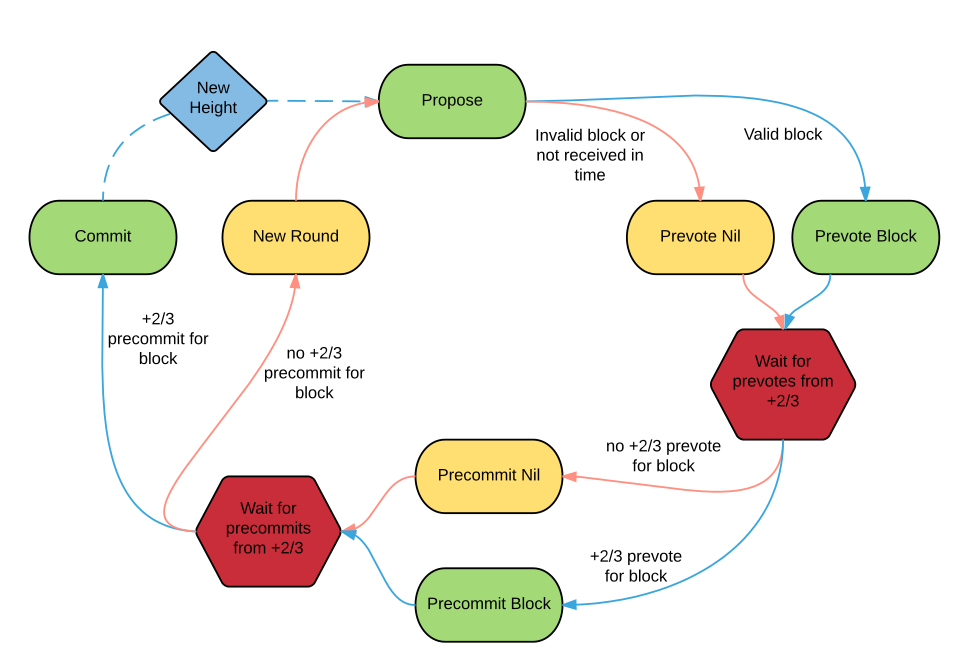
\includegraphics[width=0.8\textwidth]{img/tendermint.png}}
%\caption{Basic Tendermint operation \cite{buchman2016tendermint}}
%\label{Idur}
%\end{figure}


\begin{itemize}
    \item \textbf{Propose}

    The deterministic leader selection function indicates to each node which member of the committee is the current proposer. If a node determines that it is the leader of the current consensus instance it must generate a block, based on its received transactions, and propose it to the network.    Other nodes await the proposal.
    
    \item \textbf{Prevote}

    Once a node receives a proposal it analyzes the block's validity. If the block is valid and was sent from the correct proposer, the node agrees with the proposal and broadcasts a prevote for the block. If the block is invalid, the node prevotes nil. 

    As proposers may not send proposals in a timely manner, due to network issues or Byzantine faults, Tendermint makes use of timeouts. After processing a block, each node awaits a dynamic time interval for the next proposal.  If it is not received within this interval, the node automatically prevotes nil. This timeout is calculated locally according to pre-defined rules, allowing liveness to be maintained as long as the model assumptions hold. 

 After sending its prevote, each node awaits for a quorum. If the node receives a quorum of prevotes for the block, 
 it broadcasts a precommit for the block.   In any other case, including if the node times out when waiting for a quorum, the node 
 broadcasts precommits nil. 
    
    \item \textbf{Precommit}

The precommit phases begins as soon as the node broadcasts a precommit value. If the node receives a quorum of precommits for the block, the block is considered committed and appended to the chain, and consensus for the next block (height) is started.
 Otherwise, if a quorum cannot be reached or if the node timeouts, consensus restarts with the next proposer, in the same height but increasing round. 

\end{itemize}


A primary distinction of Tendermint is the implementation of a rotating proposer mechanism: by using a round-robin approach in which each node proposes only once, the network mitigates censorship \cite{wahrstatter2024blockchain}. % and ensures that an honest proposer eventually assumes leadership. 

Furthermore, unlike PBFT, Tendermint is designed for environments where unknown participants can join. To protect against Sybil attacks\cite{douceur2002sybil}, where a malicious actor might otherwise flood the network with nodes to gain control, the protocol integrates a Proof of Stake (PoS) mechanism. %This economic barrier shifts this is the last candidate.  next esc will revert to uncompleted text. he security assumption from a count of nodes to a distribution of wealth: the system remains secure as long as less than one-third of the total staked tokens are held by Byzantine actors. 
Participants receive rewards for consensus participation, while detected malicious behavior results in the destruction or reduction of their stake via slashing. This design effectively increases the cost of subversion, making it expensive for an adversary to acquire a quorum.

\section{Taxonomy of leader selection strategies}
\label{sec:taxonomy}
%\section{Related Work}

Several works have explored performance-aware leader selection in Byzantine fault-tolerant consensus.
Existing proposals differ substantially in both their objectives and integration strategies. 
To better position our contribution, we classify prior work along seven dimensions (see Table~\ref{related}): 
\textbf{(I) Score Representation}, distinguishing between continuous scores and discrete node classes; 
\textbf{(II) Committee Eviction,} indicating whether nodes may be removed from the active committee; 
\textbf{(III) Evaluation Metrics}, describing the information used to estimate node quality; 
\textbf{(IV) Communication Overhead}, indicating whether the mechanism requires additional protocol messages or coordination phases; 
\textbf{(V) Decoupled Architecture}, capturing whether the optimization is implemented independently from the consensus core and can therefore be reused across different SMR protocols; 
\textbf{(VI) Continuous Evaluation}, indicating whether node quality is continuously updated during execution; and 
\textbf{(VII) Rotation Policy}, describing whether proposer rotation remains active after optimization.

Most related proposals are derived from PBFT-style primary-backup architectures and therefore focus on improving view-change behavior after detecting a slow or faulty leader (e.g., \cite{eischer2018latency, shan2025grouped, zhang2024prestigebft, zhu2025rgpbft}). 
In these systems, node differentiation primarily serves as a ranking mechanism for selecting replacement leaders after a disruption. 
Proposer optimization is often reactive rather than adaptive.

A second recurring characteristic is the reliance on committee eviction to sustain performance (e.g., \cite{du2020performance, huang2023improved, qiao2024enhancing, wen2025mapbft, zhao2022pbft}). 
These approaches remove nodes considered slow, unstable, or suspicious from the active consensus set. 
While effective at increasing throughput in controlled environments, committee reduction introduces a direct trade-off between performance and Byzantine resilience. Removing slow but correct nodes reduces the effective committee size, thereby lowering the maximum number of Byzantine faults the system can tolerate. 
Moreover, modern blockchain deployments already incorporate mechanisms to detect and exclude malicious validators, making additional performance-oriented eviction layers potentially redundant and operationally risky.


%\vspace{-3mm}
\begin{table}[h!]
\centering
\begin{threeparttable}
 \scriptsize 
\newcolumntype{P}[1]{>{\centering\arraybackslash}p{#1}}
\newcolumntype{M}[1]{>{\centering\arraybackslash}m{#1}}
\begin{tabular}
{|M{0.9cm}|M{0.6cm}|M{0.8cm}|M{5cm}|M{1cm}|M{0.8cm}|M{0.8cm}|M{0.8cm}|}
\hline 
\rotatebox{90}{\textbf{Algorithm} } & 
\rotatebox{90}{\shortstack{\textbf{Score}\\\textbf{Type}} } & 
\rotatebox{90}{\shortstack{\textbf{Committee}\\\textbf{Eviction}} } &
\rotatebox{90}{\shortstack{\textbf{Evaluation}\\\textbf{Metrics}} } & 
\rotatebox{90}{\shortstack{\textbf{Communic.}\\\textbf{Overhead}} } &
\rotatebox{90}{\shortstack{\textbf{Decoupled}\\\textbf{Architecture}}  } & 
\rotatebox{90}{\shortstack{\textbf{Continuous}\\\textbf{Evaluation}} } & 
\rotatebox{90}{\shortstack{\textbf{Rotation}\\\textbf{Policy}} }\\ 
\hline
\cite{du2020performance} &
C&
Y &
Consensus participation and proposal success ratio &
Y &
Y &
Y &
N\\
\hline

\cite{eischer2018latency} &
C&
N&
Per-node consensus latency measured through active probing by clients&
Y\tablefootnote{Multiple consensus.}&
Y &
N &
N \\
\hline

\cite{huang2023improved} &
D&
Y &
Composite reputation derived from performance and participation &
Y &
N &
Y &
N\\
\hline

\cite{qiao2024enhancing} &
D&
Y &
Latency, availability, activity level, and consensus contribution &
Y &
N &
Y &
N\\
\hline

\cite{shan2025grouped} &
D&
N &
Behavioral classification and response-time analysis &
Y &
N &
Y &
N\\
\hline

\cite{wen2025mapbft} &
C&
Y &
Latency measurements combined with reputation signals &
Y &
N &
Y &
N\tablefootnote{The primary is the node with the most voting power \cite{wen2025mapbft}. If voting power changes, a new node can become the primary even without suspected failure. However, the algorithm does not perform intentional leader rotation.}\\

\hline
\cite{yu2024adaptive} &
C&
N &
Observed leader throughput during evaluation windows &
N &
Y &
N &
N\\
\hline

\cite{zhang2024prestigebft} &
C&
N&
Historical leader success, measured by committed blocks&
Y&
Y\tablefootnote{For systems without leader rotation.} &
Y &
N \\
\hline

\cite{zhao2022pbft} &
D&
Y &
Binary success/failure outcomes of consensus participation &
N &
N &
Y &
N\\
\hline

\cite{zhu2025rgpbft} &
C&
N &
Consensus participation consistency, and failure frequency &
Y &
N &
Y &
N\\
\hline

This paper &
C&
N &
Consensus duration&
Y &
Y &
Y &
P\\
\hline

\end{tabular}
\caption{Taxonomy of leader selection strategies.}
\begin{tablenotes}
\small
\item Legend: Continuous (C) scores allow fine-grained proposer differentiation, while Discrete (D) scores classify nodes into categories. Committee Eviction indicates whether nodes may be removed from the active consensus committee. Proportional (P) rotation biases proposer frequency according to performance, whereas No rotation (N) maintains the primary/proposer until a view change is proposed.
\end{tablenotes}
\label{related}

\end{threeparttable}
\end{table} 

The surveyed literature also differs in how it treats proposer fairness. 
Many PBFT-derived optimizations effectively converge toward fixed or weakly rotating leaders, increasing susceptibility to censorship and centralization. 
%Yu et al. \cite{yu2024adaptive} partially address this issue by enforcing equal rotation among nodes above a performance threshold. 
Our approach instead adopts proportional prioritization: higher-performing nodes are selected more frequently, while all nodes remain eligible proposers. This preserves continuous rotation while still exploiting topology-aware performance asymmetries.
%[OUR APPROACH CAN, DEPENDING ON THE CONFIGURED VALUES (E.G. ALLOWING SCORE TO BE UP TO +-100\% OF STAKE), REMOVE NODES FROM ROTATION (BUT KEEP THEM IN THE COMMITTEE). THIS IS INTENTIONAL AND ALLOWS FOR MAXIMUM THROUGHPUT AT THE COST OF CENSORSHIP RESILIENCE]

Finally, existing work generally treats proposer performance as an abstract property associated with computational speed or node responsiveness, with limited investigation into how network topology shapes consensus execution. 
Our experiments show that proposer placement directly affects overall consensus latency, influencing the duration of subsequent protocol phases. 
In geo-distributed deployments, proposer location therefore becomes a first-order determinant of consensus efficiency rather than merely a secondary implementation detail.

Table~\ref{related} highlights two dominant trends in prior work: (i) performance optimization through committee reduction, and (ii) tightly coupled protocol-specific leader management. 
Our approach differs in that it preserves the full committee and the original Byzantine threshold while continuously adapting proposer frequency based on observed consensus performance. 
Unlike eviction-based strategies, proposer prioritization improves throughput without sacrificing resilience or requiring invasive protocol modifications.



%This reliance on PBFT also creates an evaluation gap in the literature. 
%%Existing comparisons frequently focus on legacy PBFT baselines under heavy Byzantine attacks. Consequently, 
%It remains unclear how modern production-grade SMR systems with native Byzantine removal (such as Tendermint or HotStuff) would benefit from these proposed optimizations.
%%
%Additionally, while these primary-replica systems inherit a susceptibility to censorship, the surveyed literature largely leaves this vulnerability unaddressed. A notable exception is the work by Yu et al. \cite{yu2024adaptive}, which mitigates censorship by enforcing a uniform rotation among all nodes that exceed a baseline performance threshold. 
%
%In contrast, our approach balances performance and censorship resistance by biasing the leader rotation toward high-performing nodes. This design enhances throughput while preserving continuous rotation across the committee. Tailored specifically for modern SMR architectures, our solution maintains original Byzantine fault-tolerance bounds and acts as a non-invasive plugin that optimizes proposer selection without modifying the underlying consensus algorithm.
%
%Finally, a recurring limitation across prior work is the superficial treatment of consensus latency. The assumption that computationally weak or topologically distant nodes degrade performance is often accepted without empirical investigation. Our experiments challenge this oversimplification, demonstrating that node-to-node network latency is a critical factor that dictates not only individual step durations, but also the dynamic composition of the quorums that actively drive consensus.

\section{Understanding the Impact of Proposer Location}
\label{sec:impact}

This section investigates how proposer’s network latency relative to other nodes affects overall consensus performance. We evaluate: (i) the measurable impact on consensus duration; (ii) effects on individual step durations; (iii) influences on quorum formation; and (iv) potential throughput gains using optimized proposer placement. 

We conducted experiments on the CloudLab\footnote{\url{https://cloudlab.us/}} testbed using 13 m510\footnote{\url{https://docs.cloudlab.us/hardware.html\#(part.cloudlab-utah)}} nodes. Each node emulated a distinct AWS zone, with inter-node latencies\footnote{\url{https://github.com/cometbft/cometbft/blob/v2.x/test/e2e/pkg/files/aws-latencies.csv}} injected via the \texttt{tc}\footnote{https://www.man7.org/linux/man-pages/man8/tc.8.html} (traffic control) utility to represent a realistic geo-distributed topology. The study utilized the Malachite implementation of the Tendermint protocol. Each execution lasted five minutes, including a 30-second warm-up and 15-second cool-down, with clock synchronization maintained via NTP to ensure deviations remained below 10ms.

Our experimental methodology followed a sequence of targeted tests. First, a \textit{sanity check} was performed using a 4-node topology with a uniform 100ms latency. The results showed negligible variation ($< 1.6\%$) across proposers, both for fixed and rotating strategies, confirming that any subsequent performance discrepancies were strictly due to network topology.  Also, we observed no impact in switching proposers at each decision or after a number of decisions.  For better legibility, we show figures with results switching proposers every 10 decisions.

\subsubsection{Proposer Impact on Consensus Duration.}
The primary metric for evaluating proposer location is the total time elapsed from the initial proposal to the final decision. In our 13-node heterogeneous topology, we observed that the physical location of the proposer is a dominant factor in system performance. As illustrated in Figure \ref{Idur}.a, consensus durations measured at proposers range from a minimum of 0.47s to a maximum of 0.73s depending on which node lead the round, a 40\% performance gap.   Figure \ref{Idur}.b depicts the latency from proposal to decision as measured at each node, showing that impact on termination latency at each node is also impacted by the proposer.
%demonstrates that even without computational bottlenecks, the network's "center of gravity" significantly dictates the speed of the entire system.

\begin{figure}
     \centering
     \begin{subfigure}{0.95\textwidth}
         \centering
         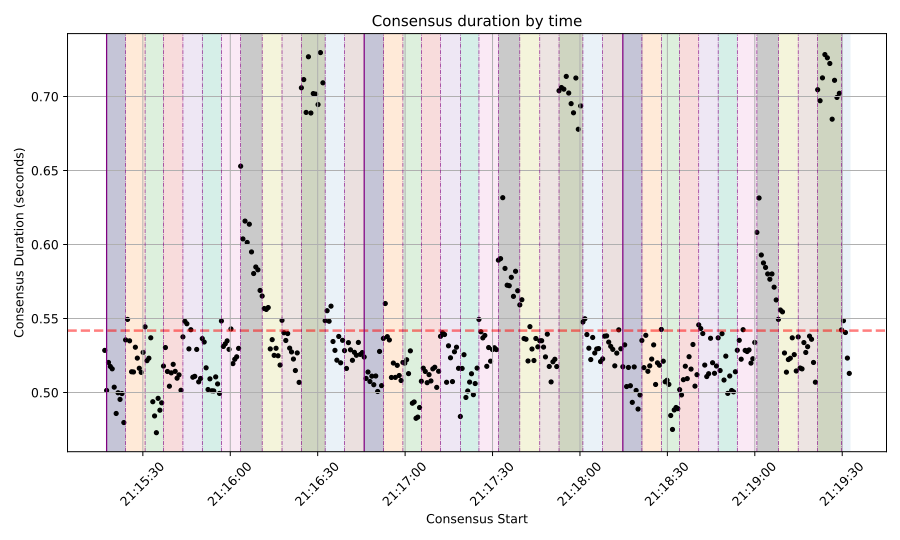
\includegraphics[width=\linewidth]{svgi/10xconsensusDurationLeader.svg.png}
         %\includesvg[width=\linewidth]{svg/10xconsensusDurationLeader.svg}
         \caption{Latency from propose to decide measured at each proposer}
         \label{fig:1a}
     \end{subfigure}
     \\
     \begin{subfigure}{0.95\textwidth}
         \centering
         % Cor nas linhas, ruim de ver de longe
         %\includesvg[width=\linewidth]{svg/10xoptdecidedDeviationBlocktimeLeader.svg}
         %\includesvg[width=\linewidth]{svg/10xoptbackdecidedDeviationBlocktimeLeader.svg}
         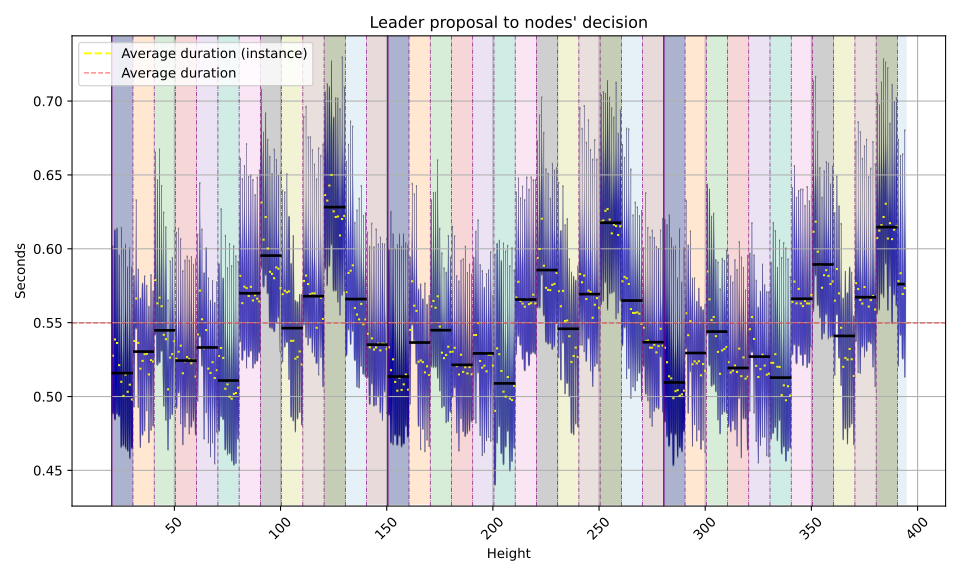
\includegraphics[width=\linewidth]{svgi/10xoptbackdecidedDeviationBlocktimeLeader.svg.png}
         \caption{Each vertical line refers to
a consensus instance and is composed by plots with the consensus latency of each node}
         \label{fig:1b}
     \end{subfigure}
     \caption{(a) Consensus latency at proposer and (b) Consensus latency at all nodes.
     10 instances per proposer, divided by vertical dotted lines. Solid line indicates a new round through same proposers - repeating the pattern, each proposer has a different color. }
     \label{Idur}
\end{figure}

CDF da figura 1.a

cdf da figura 1.b

figura 2 -  nao se justifica

titulo p 4

tail latency nos resultados



\subsubsection{Proposer Impact on Consensus Steps.}
After the proposal, further communication steps are all-to-all. While the time to receive a quorum, in all-to-all communication phases, theoretically depends on the location of each receiver node, 
%in proposer-based algorithms are theoretically symmetric, 
we investigated whether the proposer's location could influence such steps.
%We define \textit{prevote} duration as the interval from proposal receipt to quorum collection, and \textit{precommit} duration as the time from prevote quorum to precommit quorum.
%
Fig.\ref{fig.steps} displays individual prevote (a) and precommit (b) step durations, showing that proposer location measurably also impacts the latency of these consensus phases.   

\begin{figure}
     \centering
     \begin{subfigure}{0.95\textwidth}
         \centering
         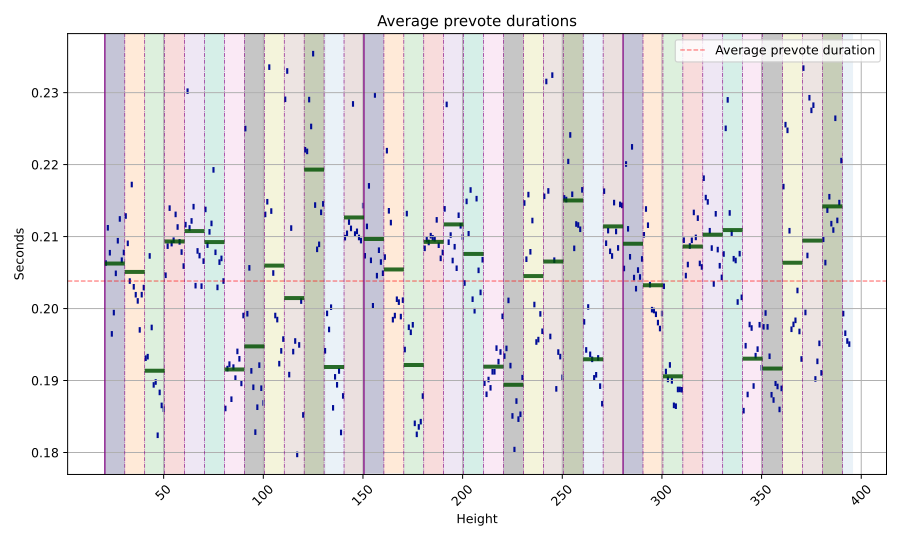
\includegraphics[width=\linewidth]{svgi/10xlimStepPrevoteLeader.svg.png}
         \caption{}
         \label{fig:2a}
     \end{subfigure}
     \\
     \begin{subfigure}{0.95\textwidth}
         \centering
         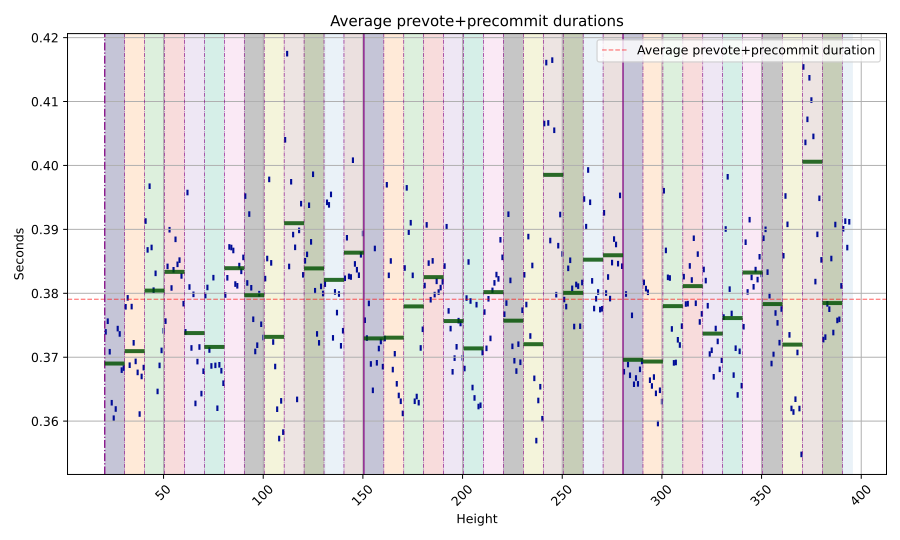
\includegraphics[width=\linewidth]{svgi/10xlimStepPrevotePrecommitLeader.svg.png}
         \caption{}
         \label{fic:2b}
     \end{subfigure}
     \caption{(a) For each instance a we measure each nodes latencies from receiving a proposal until a quorum of prevotes is received. We then calculate the per-proposer mean (green) and global mean (red).  \\
     (b) The same for each nodes latencies from receiving the proposal until a quorum of precommits is received.}
     \label{fig.steps}
\end{figure}


\subsubsection{Influences on Quorum Formation.}
One hypothesis to better understand the previous result is that 
a proposer impacts the formation of quorums, which in turn affects step durations.
%Suppose a proposer $p$ close to a node $n_1$, which is distant from $n_2$.  $n_1$ would quickly respond $p$'s $propose$ message with $prevote$ to all nodes, possibly reaching $n_2$ before other nodes messages to $n_2$, i.e. $n_2$'s prevote quorum includes a distant node $n_1$. 
To check this, we computed and evaluated the quorums built at each node, rotating the whole set of proposers several rounds.   We observed a 98\% consistency in quorum composition when the same node acted as proposer. Nodes geographically closer to the proposer receive the proposal faster and, consequently, their votes are the first to arrive and form the $prevote$ quorum.
%
As stated in the Tendermint specification, if a farther node manages to join another node’s prevote quorum, that second node will wait for that node in the $precommit$ step even if a faster quorum is reached (this is intended for Proof of Stake rewards).   This means that in the precommit phase, a specific node cannot progress with it's ideal quorum (set of closest nodes), negatively impacting latency and throughput.   This also leads to the high consistency among prevote and precommit quorums in a specific node.

\subsubsection{Throughput Gains via Proposer Placement}
The final aspect of our analysis compared the standard round-robin rotation against a fixed-proposer configuration using topologically "ideal" nodes. The results confirm that by steering the protocol to favor leaders with lower median latency to the rest of the network, the system achieves significantly higher sustained throughput.

 [??? bla bla ... tem que colocar numeros aqui !!!!  e fazer o texto mais sucinto ]

This gain is achieved without modifying the underlying BFT safety logic, proving that performance-aware leader selection is a viable optimization for geo-distributed blockchains.



\section{Algorithm Proposal}
\label{sec:algorithm}

As shown in the previous section, the position of a proposer does impact consensus performance. From this observation we devise an approach to dynamically adjust the frequency that each participant becomes proposer, favoring faster ones, and thus enhancing overall consensus performance. The proposed approach poses the following assumptions to the underlying consensus algorithm:  
\begin{description}
    \item[A.1] it uses rotating proposer and provides means to record the future sequence of proposers (or parameters to calculate it); 
    \item[A.2] it has a deterministic function used at each node to calculate the next proposer.   We call this function \textit{nextProposer}.  For instance, with PoS, the next proposer is a function of the known stakes from each participant. 
\end{description}

The proposed mechanisms should ensure the following basic properties:
\begin{description} 

    \item[P.1] the underlying consensus algorithm properties are preserved;     
    %For instance, it does not modify the composition of the consensus committee, unlike some of the related works; 

    \item[P.2] disregarding stake, or with a uniform stake distribution, proposer nodes with faster (slower) decisions become proposers proportionally more (less) often;

    \item[P.3] changes in a node's relative performance over time lead to respective adaptation of its frequency as proposer;  

    \item[P.4] every node eventually becomes proposer.
\end{description}

And the byzantine fault-tolerance properties:
\begin{description} 
   
    \item[P.5] dishonest nodes do not impose an arbitrary sequence of proposers;
    
    \item[P.6] dishonest nodes do not hinder the differentiation of faster/slower nodes. 

\end{description}

To achieve the desired properties, three concurrent, continuous mechanisms are proposed:
\begin{description} 
    \item[M.1] every node samples the latency and locally classifies each other node;
    
    \item[M.2] every node collaborates to generate consistent global classifications;
    
    \item[M.3] every node uses the global classification to calculate and adopt a new sequence of proposers.   
\end{description}

\subsection{M.1 - Sampling and classifying nodes}

While the techniques for sampling and classifying nodes may vary, we describe here one with low computational cost, yet effective in our experiments. 
%
Each node continuously samples the latency of the successive consensus heights.  This measure is local, comprising the time elapsed from the start of the current consensus (e.g. Tendermint's propose) to it's decision (e.g. Tendermint's decided).   Since each consensus height is associated to a known proposer, the sample denotes that proposer's performance.  

\paragraph{Set of latency samples $L$.} Let $L$ be a set with the $k$ last consensus latency samples taken by a node, $k$ being a configuration parameter.  At any time, the average consensus latency $\bar{L}$ is known at the node.

\paragraph{A parameter $T \in {0..1}$} defines a threshold for node classification against the average latency $\bar{L}$. A latency sample $s$ for a consensus instance can be considered $fast$ if $s < \bar{L} \times (1-T)$; $slow$ if $s > \bar{L} \times (1+T)$; and none ($\bot$) otherwise.  
%
The purpose of $T$ is primarily to deal with short-term variations (jitter) in the observed performance of nodes,
reducing the alternation of "fast" and "slow" classifications for a same node. 
It achieves that by creating a neutral zone around the system average where proposal speed is considered neither "fast" nor "slow". The lower the $T$ the more non-$\bot$ decisions are achieved, at the cost of increasing sensitivity to transient latencies. The higher the $T$ the more resistant it is, but at the cost of less non-$\bot$ decisions. %$T$ must be a value $\geq0$, with an ideal minimum $T$ approximating how much consensus can vary due to noise in percents  ...???? 

\paragraph{Denote $c_h \in \{ fast, \bot, slow \}$} the above classification for consensus height $h$.

\subsection{M.2 - From local to global classifications}

Now, the challenge is to derive, from these local classifications, meaningful global decisions with respect to which nodes are considered fast, slow, or none.  
%
Our algorithm is based on three steps: \textit{vote}, \textit{choice}, and \textit{write}.   We propose here that these steps are carried out with the underlying consensus algorithm messages and steps, having an implicit trigger associated with it.  Our discussion uses Tendermint, with the following behavior at each node:

\begin{itemize}
\item \textit{Vote:} upon start of height $h+1$, send $\langle vote,h,c_h \rangle$ to all other nodes.  $c_h$ is the classification already discussed regarding consensus instance at height $h$.   
%
This vote is sent along with the first message for height $h+1$ to all other nodes  (e.g. Tendermint's prevote).  
Voting lasts until the decision for height $h+1$.  
The reason for using the decision as a limit is twofold. First, the synchronization eases the integration of the mechanism and reuse of messages. %, ensuring scores are updated in a timely manner. 
And second, it allows to gather additional votes beyond the quorum needed to advance the underlying consensus phase.

\item \textit{Choice:} upon start of height $h+2$, if a quorum of $2f+1$ \textit{vote} messages for a same non-$\bot$ $value$ is reached,  send a signed message $\langle choose,h,value \rangle_{sig}$ to all other nodes.   Otherwise, send a $\langle choose,h,\bot \rangle$ non-signed message. 
As with the voting step, the $choose$ message is sent along the first message for the next height ($h+2$)
and its reception lasts until the decision for that height.    


\item \textit{Write:}  Upon start of height $h+3$, nodes gather the chosen values and decide the value to write, called $decided_h$.   
%
If a node has received a quorum of $2f+1$ 
\textit{choose} messages for a same non-$\bot$ value,
the node decides that value. 
Otherwise decides the default value of $\bot$.

The proposer of height $h+3$ $write$s with the proposal: the $decided_h$ value; if $decided_h \neq \bot$, the quorum of signed choices; and the updated scores of all nodes.  Scores are discussed in Section \ref{subsec:scores}.  If $decided_h = \bot$, there is no need to record the quorum of signed choices.  
% COMPLEMENTAR ISSO ?
If a dishonest proposer node may omit, not writing a non-$\bot$ value, an honest next proposer may write the value with the quorum of signed choices justifying it.
Each proposer node thus keeps a window of $decided_h$ with their respective set of signed choices justifying the value.

Any node, upon receiving a proposal which can be accepted by the underlying consensus algorithm, adds the following: if $decided_h = \bot$, accepts it;  if $decided_h \neq \bot$, accepts if signatures are successfully verified. If not accepted, evidence of dishonest behavior is generated.

%A node only votes for the proposal (e.g. Tendermint's block) if the decided value and the updated scores in the proposal match its own values. This is necessary to prevent Byzantine proposers from simply ignoring the last vote. 

\end{itemize}

Note that all steps can happen simultaneously. During a consensus for height $h$, there can be an ongoing $vote$ step for height $h-1$, a $choice$ step for height $h-2$, and a $write$ step for $h-3$. %This only implies in two extra values (vote and choice) in each node's first message of that height. 


\subsection{M.3 - Continuous scoring and proposer prioritization}
\label{subsec:scores}

So far we have discussed how each consensus instance $h$, and it's associated proposer $n$, is associated with a classification $decided_h$ in $\{fast, \bot, slow \}$ known by all nodes.
%
Now we address how this classification can be used to steer proposer selection.   There are two main aspects to consider: 
(i) assuming a \textit{nextProposer} function using the $stake_n$ of each node $n \in \Pi$ to decide the proposer sequence, how can we extend the function to prioritize faster nodes;
(ii) considering that the relative performance of nodes may vary over time, due to several external factors, how the prioritization adapts to the changing relative performance of proposers.

\paragraph{We define $weight_n$ for each node $n \in \Pi$,} as: 
\begin{equation} 
\label{eq.weight}
weight_n = stake_n \times [1 + ( C \times nomalizedScore_n) ]
\end{equation}

Instead of inputting $stake$, the \textit{nextProposer} function is used with $weight$.   $C$ and $nomalizedScore_n$ are discussed next.


\paragraph{We define the input parameter $C$, the contribution of score,} to denote how much each node's score modifies its stake. This ensures that, in systems where different stake values are possible, the score remains proportional to those different stakes. 
$C=0$ disables the score algorithm and values $\geq1$ would allow nodes to be removed from the proposer pool. $0 < C < 1$ keeps all nodes in the choice and allows to differentiate them by performance.  The higher the $C$ the more performance is valued to choose the next proposer.  
%
For instance, $C=0.3$ would limit the $weight$ to $\pm30\%$  of each node's stake, leading to a $weight_n$ in the interval of $[0.7*stake_n, 1.3*stake_n]$. 

\paragraph{We now define $score_n$, $\alpha$, $\beta$ and $M$.}

We call $decided_n$ a value in $\{ -1, 0, 1 \}$ as $decide_h$ is respectively $\{ slow, \bot, fast \}$. 
A $score_n$ of each node $n \in \Pi$ is initialized to 0.
Each time a new $decided_n$ value is available, $score_n$ is updated as: 
\begin{equation} 
\label{eq.score}
score_n' = trunc_{[-M..M]}(\beta*score_n + \alpha*decided_n )
\end{equation}
%
\paragraph{$\beta$ denotes how fast older decisions decay their impact on score.}
$\beta$ is a value in $0..1$ 
%and serves to decrease the value of older decisions in favor of newer ones.   This is one measure to
and serves to adapt the prioritization of nodes to current observed performance.   It adjusts how quickly the score returns to zero with only $\bot$ decisions.

\paragraph{$\alpha$ denotes how new decisions impact the score.} 
$\alpha$ is a positive value, being a step in the modification of score. 
A higher $\alpha$ will move score faster, making score more sensitive to performance oscillations.   
If there are many non-$\bot$ decisions we can afford a small step, but if the number of non-$\bot$ decisions is small we are forced to have a larger $\alpha$. 
%
With these definitions, for any $0 \leq \beta < 1$  score is within the interval $\pm \frac{\alpha}{1-\beta}$.\footnote{Derivation of this expression omitted due to size restrictions.} 

\paragraph{$M$ is a variable which informs the limits of $score$,} which is restricted to the interval $[-M,M]$.   If $M = \frac{\alpha}{1-\beta}$ it allows the full variation of scores (truncation does not take place). 

%$M$ must be a value in the interval $[0, \frac{\alpha}{1-\beta}]$, although it should ideally be equal to that limit to allow for the full resolution of scores. 



\paragraph{We now define $nomalizedScore_n$}, resulting in a value in $-1..1$,  to be used in Equation \ref{eq.weight}, as: 
\begin{equation} 
\label{eq.normalizedscore}
nomalizedScore_n =  \frac{score_n}{M} 
\end{equation}
 



%\vspace{4mm}
As mentioned, the $nextProposer$ function needs to be deterministic in a decentralized environment. Therefore,  variables \(\alpha\), \(\beta\), $M$, $C$, and $T$ must be consistent across nodes. 
%
If the consensus supports self-configuration it is also possible to self-configure the global variables according to a pre-established set of rules, e.g. increasing the $T$ if there's too much jitter and decreasing it if there's too few decisions. For systems with self-configuration, modified variables must be stored (e.g. inside a blockchain's block) so that new nodes can update their variables to match the system. 


\subsection{Correctness and Byzantine Fault Tolerance}

The proposed mechanisms should ensure the properties described in the introduction of Section \ref{sec:algorithm}.
Each one discussed next.
% \begin{description} 
%     \item[P.1] the underlying consensus algorithm properties are preserved;     
%     \item[P.2] disregarding stake, or with a uniform stake distribution, proposer nodes with faster (slower) decisions become proposers proportionally more (less) often;
%     \item[P.3] changes in a node's relative performance over time lead to respective adaptation of its frequency as proposer;  
%     \item[P.4] every node eventually becomes proposer;  
%     \item[P.5] dishonest nodes do not impose an arbitrary sequence of proposers;
%     \item[P.6] dishonest nodes do not hinder the differentiation of faster/slower nodes. 
% \end{description}

\paragraph{Argument for P.1:} 
Regarding the properties of the underlying consensus algorithm, notice that the proposed mechanisms do not modify the algorithm.   Messages and the value proposed are conservatively extended with votes and scores,  these being processed by mechanisms separated from the underlying algorithm.  The proposed mechanisms also do not prevent the progress of the underlying algorithm: whenever 
phase or height change may occur, the proposed mechanisms proceed with the values computed so far.  

The only aspect impacted is the choice of next proposer.
The structure of the function to choose the next proposer is preserved, however being parameterized with weighted stakes according to respective nodes performance, instead of stakes only. As the weighted scheme, by definition, does not nullify any stake, every node is eventually chosen as proposer. 

\paragraph{Argument for P.2:} 
As discussed in Section \ref{subsec:scores} the $score_n$ of a node $n$ increases each time it is voted $fast$, leading to a multiplication of $stake_n$ by a factor $> 1$, that then results in proportionally augmented $weight_n$.   The weights of all nodes then substitute their original stakes in the $nextProposer$ function, leading to a more frequent choice of nodes according to their weight. 

\paragraph{Argument for P.3:} 
The proposed mechanisms continuously sample consensus latencies, adjusting scores.
The $\beta$ parameter serves to decay the importance of old samples in the current score while $\alpha$ denotes the impact of new decisions.  With this, scores adapt to changing performance observations, leading to the desired impact in the $nextProposer$ choice.

\paragraph{Argument for P.4:} 
This property derives from assumption A.1 and A.2 on the $nextProposer$ function, implying that nodes are chosen as proposers proportionally to their stake, and the fact that the scoring mechanism does not annulate any stake, but differentiates them according to the node's performance.  

\paragraph{Argument for P.5:} 
A non-$\bot$ value is written if $2f+1$ nodes choose that value.  Among those, at least $f+1$, a majority, is comprised by honest nodes, by definition.  This means that dishonest nodes cannot impose a non-$\bot$ value not supported by a majority of honest ones.


\paragraph{Argument for P.6:} 
Since there are at least $2f+1$ honest nodes, if they choose the same non-$\bot$ value, 
then this value is eventually written by an honest proposer irrespective of dishonest nodes choices
or dishonest proposers omitting the value.

\paragraph{Impact of dishonest behavior while voting:}

Properties P.5 and P.6 leave room for dishonest nodes impacting the decision if
the number of honest nodes choices $hc$ for a same non-$\bot$ value is $f+1 \leq hc < 2f+1$.

However, notice that dishonest nodes choices are limited: 
%In the \textit{vote} step, each node awaits for a quorum of other nodes. 
A node only chooses a non-$\bot$ value in the \textit{choice} step if it received a quorum of that value in the \textit{vote} step. 
As any two quorums have an overlap of at least one honest node, it is impossible for there to be two conflicting quorums. At the end of this step each node will either have a quorum of the same non-$\bot$ value, or default to $\bot$ if a quorum has not been received.  In the first case, a dishonest node sending a non-$\bot$ choice contradicting the quorum value would immediately generate evidence of dishonest behavior.
%This reduces the next step into a binary decision. 
%
This means that colluding dishonest nodes may either add choices to a majority of honest nodes 
to accept their non-$\bot$ value, or not, keeping the $\bot$ decision.      
Keeping the $\bot$ decision does not harm performance,  while accepting the non-$\bot$ value
would enhance the performance observed by a majority of honest nodes.

\paragraph{Impact of dishonest behavior while proposing:}
In the role of proposer, a written non-$\bot$ value is accompanied by the signed choices justifying the quorum.
Any modification of the agreed value would generate clear evidence of misbehavior by the proposer as
different signed choices from a same dishonest node would be available at honest nodes.

A dishonest proposer may write $\bot$ (which does not need the accompanying signed choices), 
omitting a quorum of a non-$\bot$ value.   However, any honest next proposer can write the omitted 
non-$\bot$ value and the respective signed choices, proving the value.   In practice, the omission 
by the dishonest node leads just to postponing the adoption of the value.




%\section{Experimental Evaluation}
\label{sec:experiments}

To validate the proposed mechanism, we utilized an oracle-based experimental methodology. 
We first executed the Malachite protocol using standard round-robin rotation to establish a baseline. 
From the resulting logs, we simulated the score-calculation algorithm to generate an optimized proposer sequence. 
Finally, we re-executed the protocol using this new sequence to measure performance gains. This iterative process was repeated up to six times (\textit{alg-1} through \textit{alg-6}) to observe score stabilization. 

%[???  modificou o proposto antes ????   como o leitor entende ????   gastou tempo do leitor explicando la, agora muda nao sei por que...  ]  
%For these evaluations, we measured \textit{block time} rather than consensus duration, as block time accounts for the full interval from height start to decision, providing a more realistic metric for production environments.

The scoring algorithm used consistent parameters across all tests: uniform node stake, a score range $M=5$, a 50\% consensus threshold ($T=0.5$), $\alpha=3$, $\beta=0.9$, and a 100\% contribution factor ($C=1$). These values were chosen to prioritize rapid convergence in stable network conditions.

We repeated the experimentation with 3 different topologies, respectively cases A, B and C.

\subsubsection{Case A.} 
In the 13-node AWS topology, we evaluated the iterative convergence of the algorithm (\textit{alg}) against the default rotative system (\textit{def}). As shown in \textbf{Fig. \ref{alg2}}, which tracks block times across sequential runs, the high $\alpha$ value allows the scores to stabilize within four iterations. Once stabilized, the algorithm achieves an 8\% performance gain primarily by reducing the frequency of the two most distant nodes in the proposer pool. For comparison, a traditional node-removal strategy (\textit{rem-2}) achieves a slightly higher 10\% gain but incurs a critical cost: 
the two most distant nodes were excluded, reducing the committee size from $N=13$ to $N=11$, which lowers the Byzantine fault tolerance from $F=4$ to $F=3$. Our approach maintains the full committee while achieving comparable performance.

\begin{figure}[htbp]
\centerline{%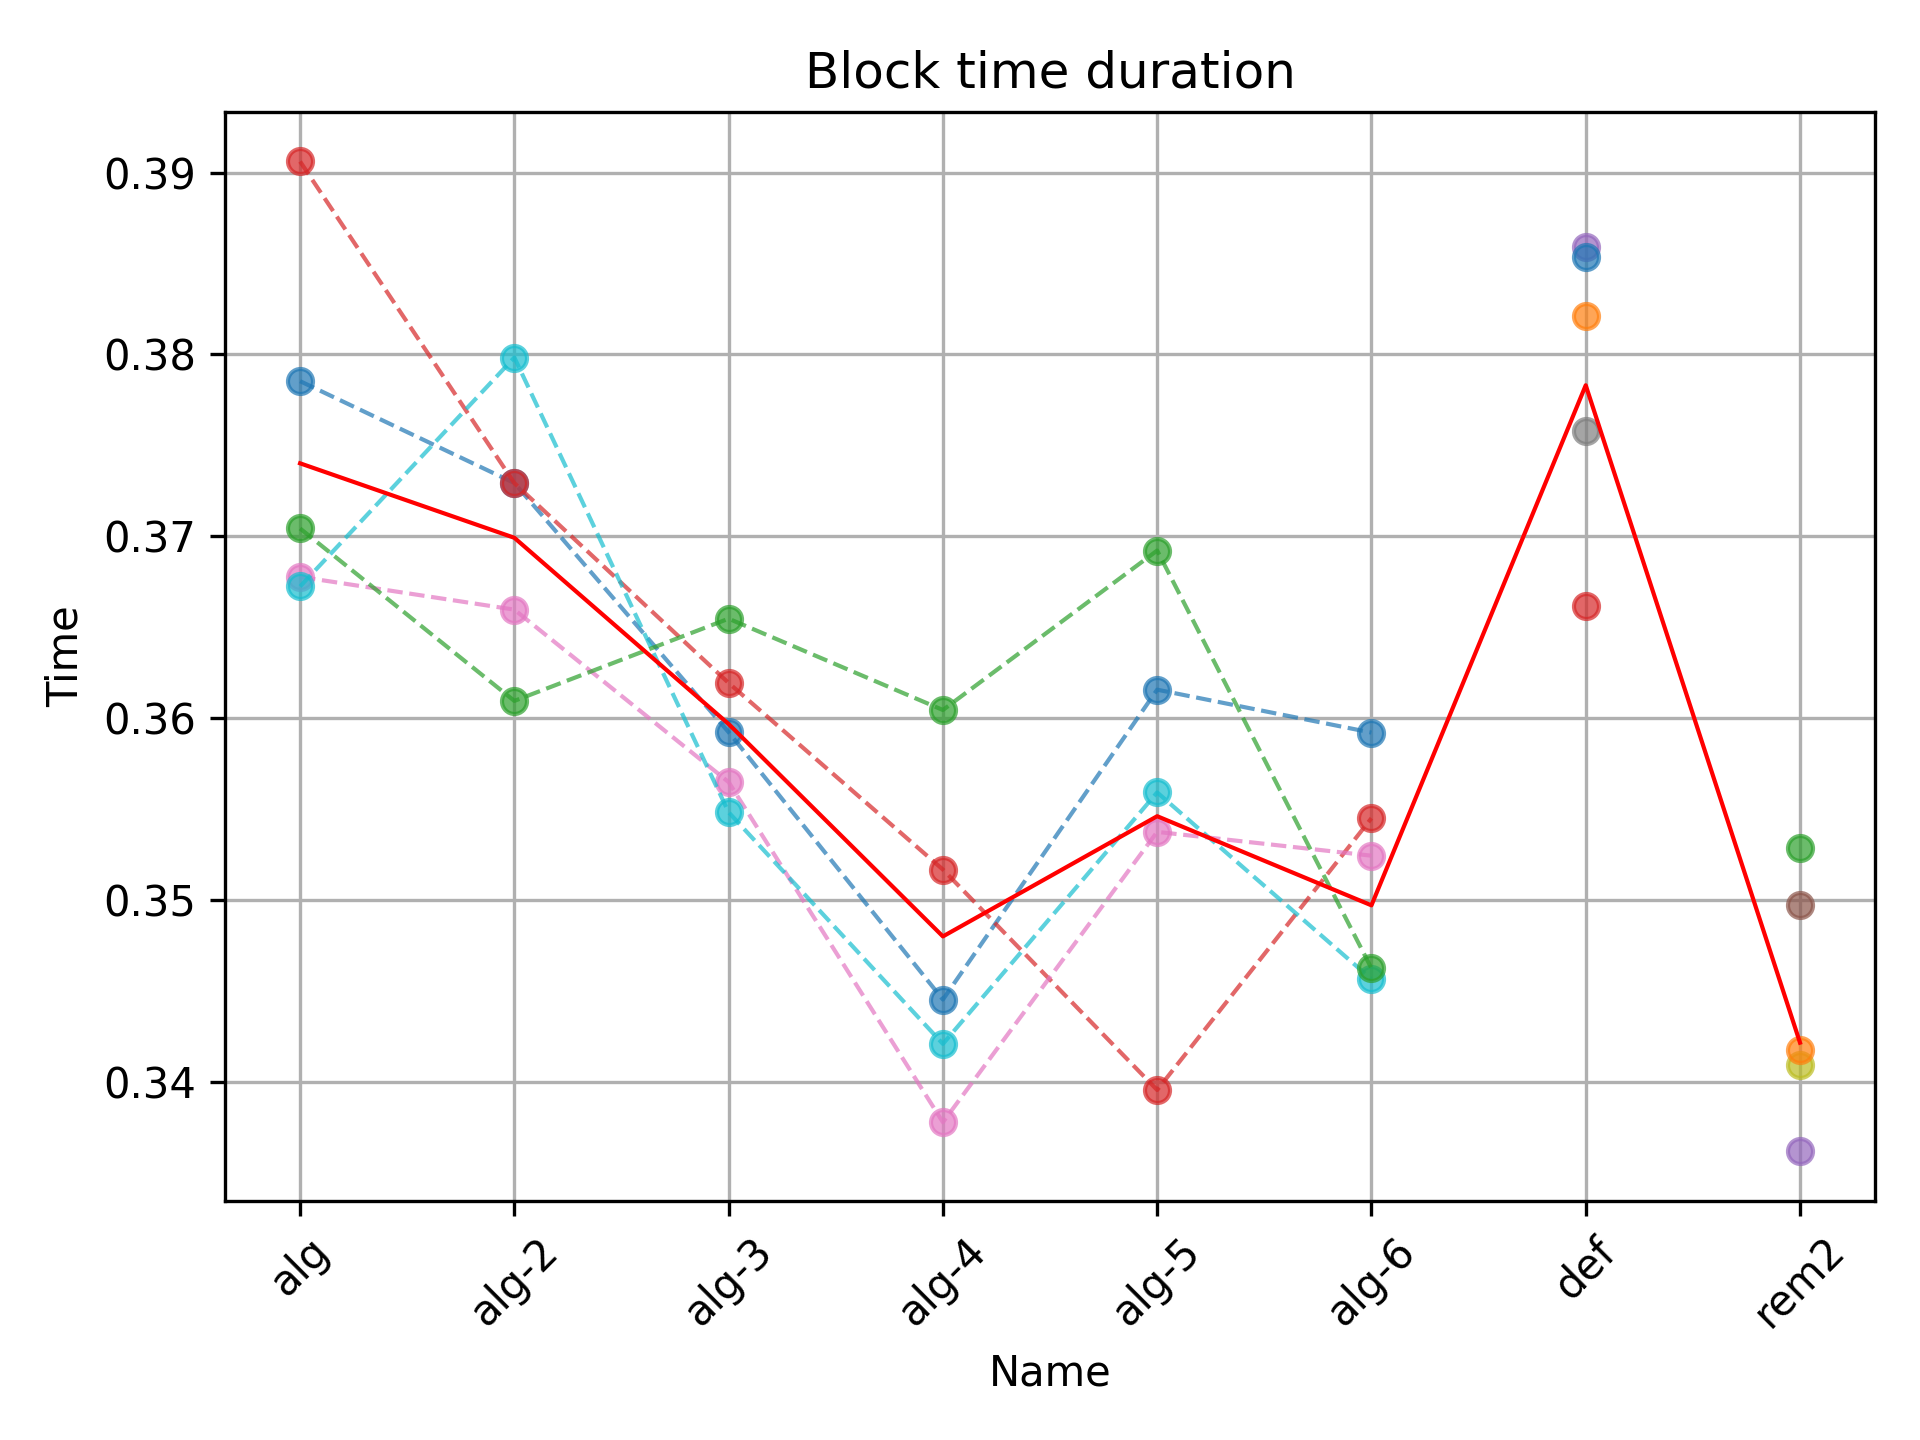
\includegraphics[width=0.5\textwidth]{img/aws13.png}}
 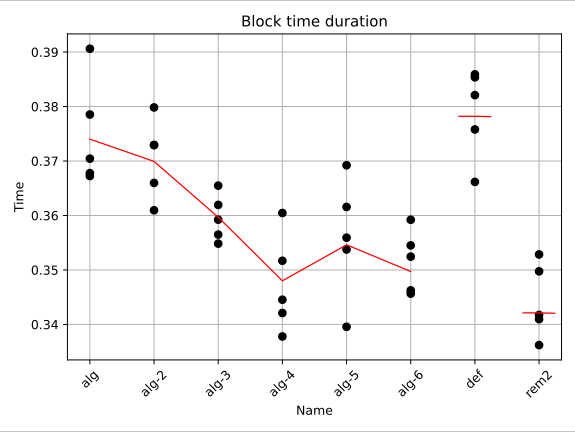
\includegraphics[width=0.6\linewidth]{svgi/awsblock.svg.png}
 %\includesvg[width=\linewidth]{svg/awsblock.svg}
}
%\centerline{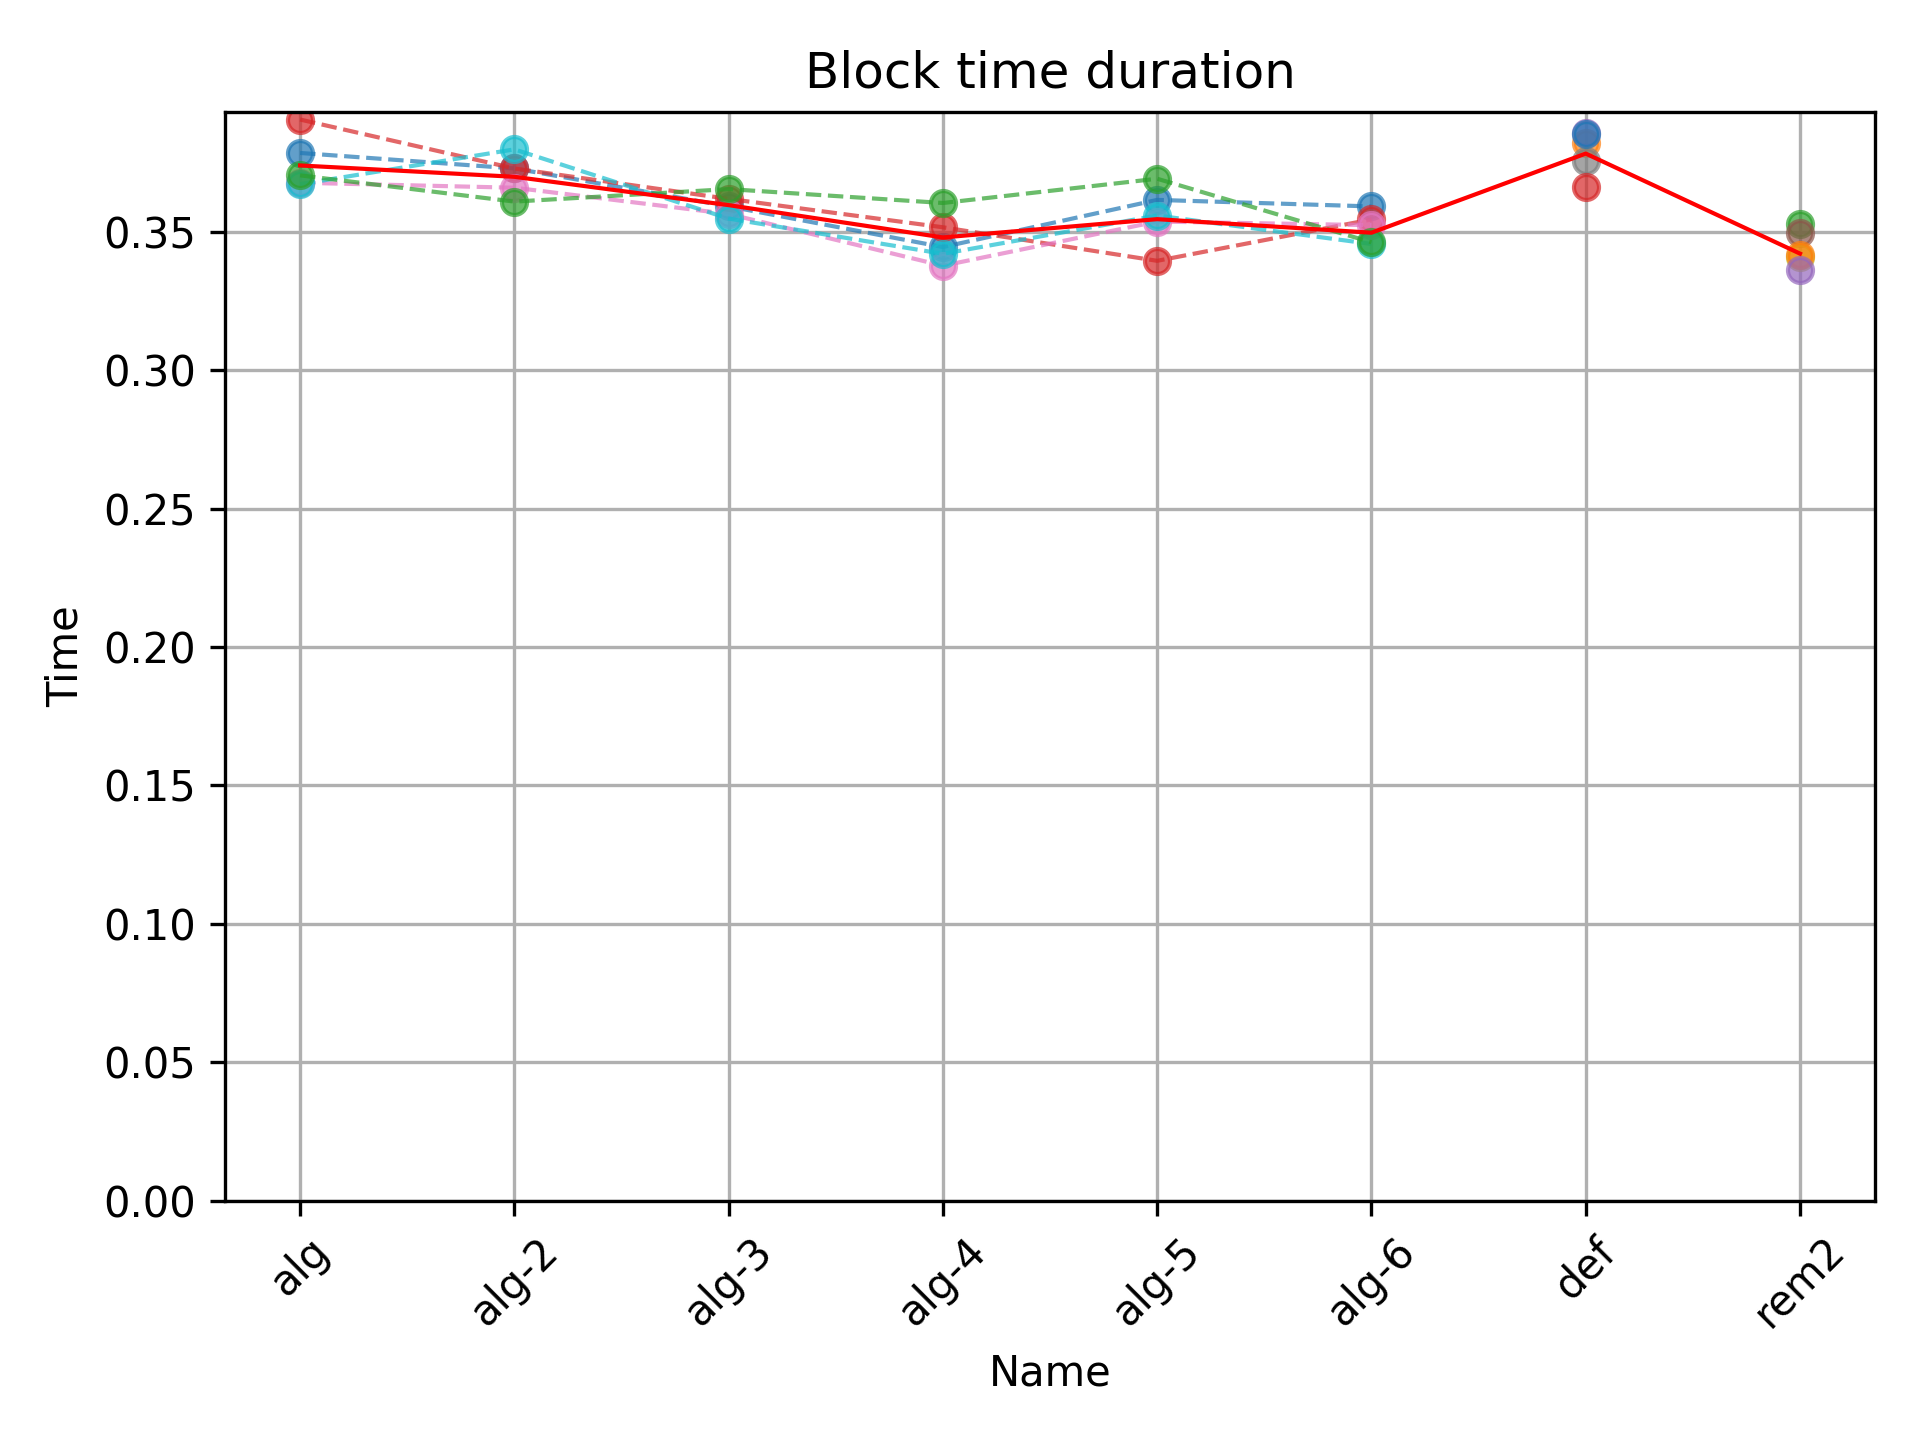
\includegraphics[width=0.3\textwidth]{img/aws13zero.png}}
\caption{Experiment with the topology used for measurements Section 3,
13 AWS zones. 5 runs (each one a plot) per configuration. Red line is the average.}
\label{alg2}
\end{figure}

\subsubsection{Case B.} To assess robustness under variable network conditions, we utilized datasets from \cite{di2025impact} to model two cases, one with 24-hour data and another with 16-month data. In the 14-node 24-hour topology (\textbf{Fig. \ref{alg24}}), the scores stabilized in only three steps, yielding a 30\% improvement on block time at the 80th percentile and a 15\% improvement at the median. This confirms that gains are topology-dependent and also that our mechanism helps filtering out long-tail latencies.

\begin{figure}[htbp]
\centerline{%\includegraphics[width=0.3\textwidth]{img/80percentileBlockDurationAvrg.png}}
 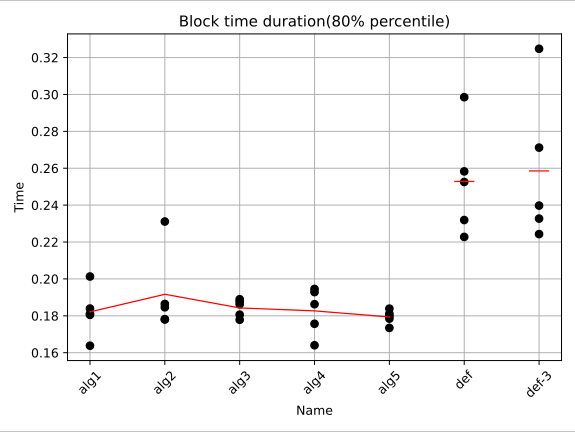
\includegraphics[width=0.6\linewidth]{svgi/dev80th.svg.png}
 %\includesvg[width=\linewidth]{svg/dev80th.svg}
 }
 
%\centerline{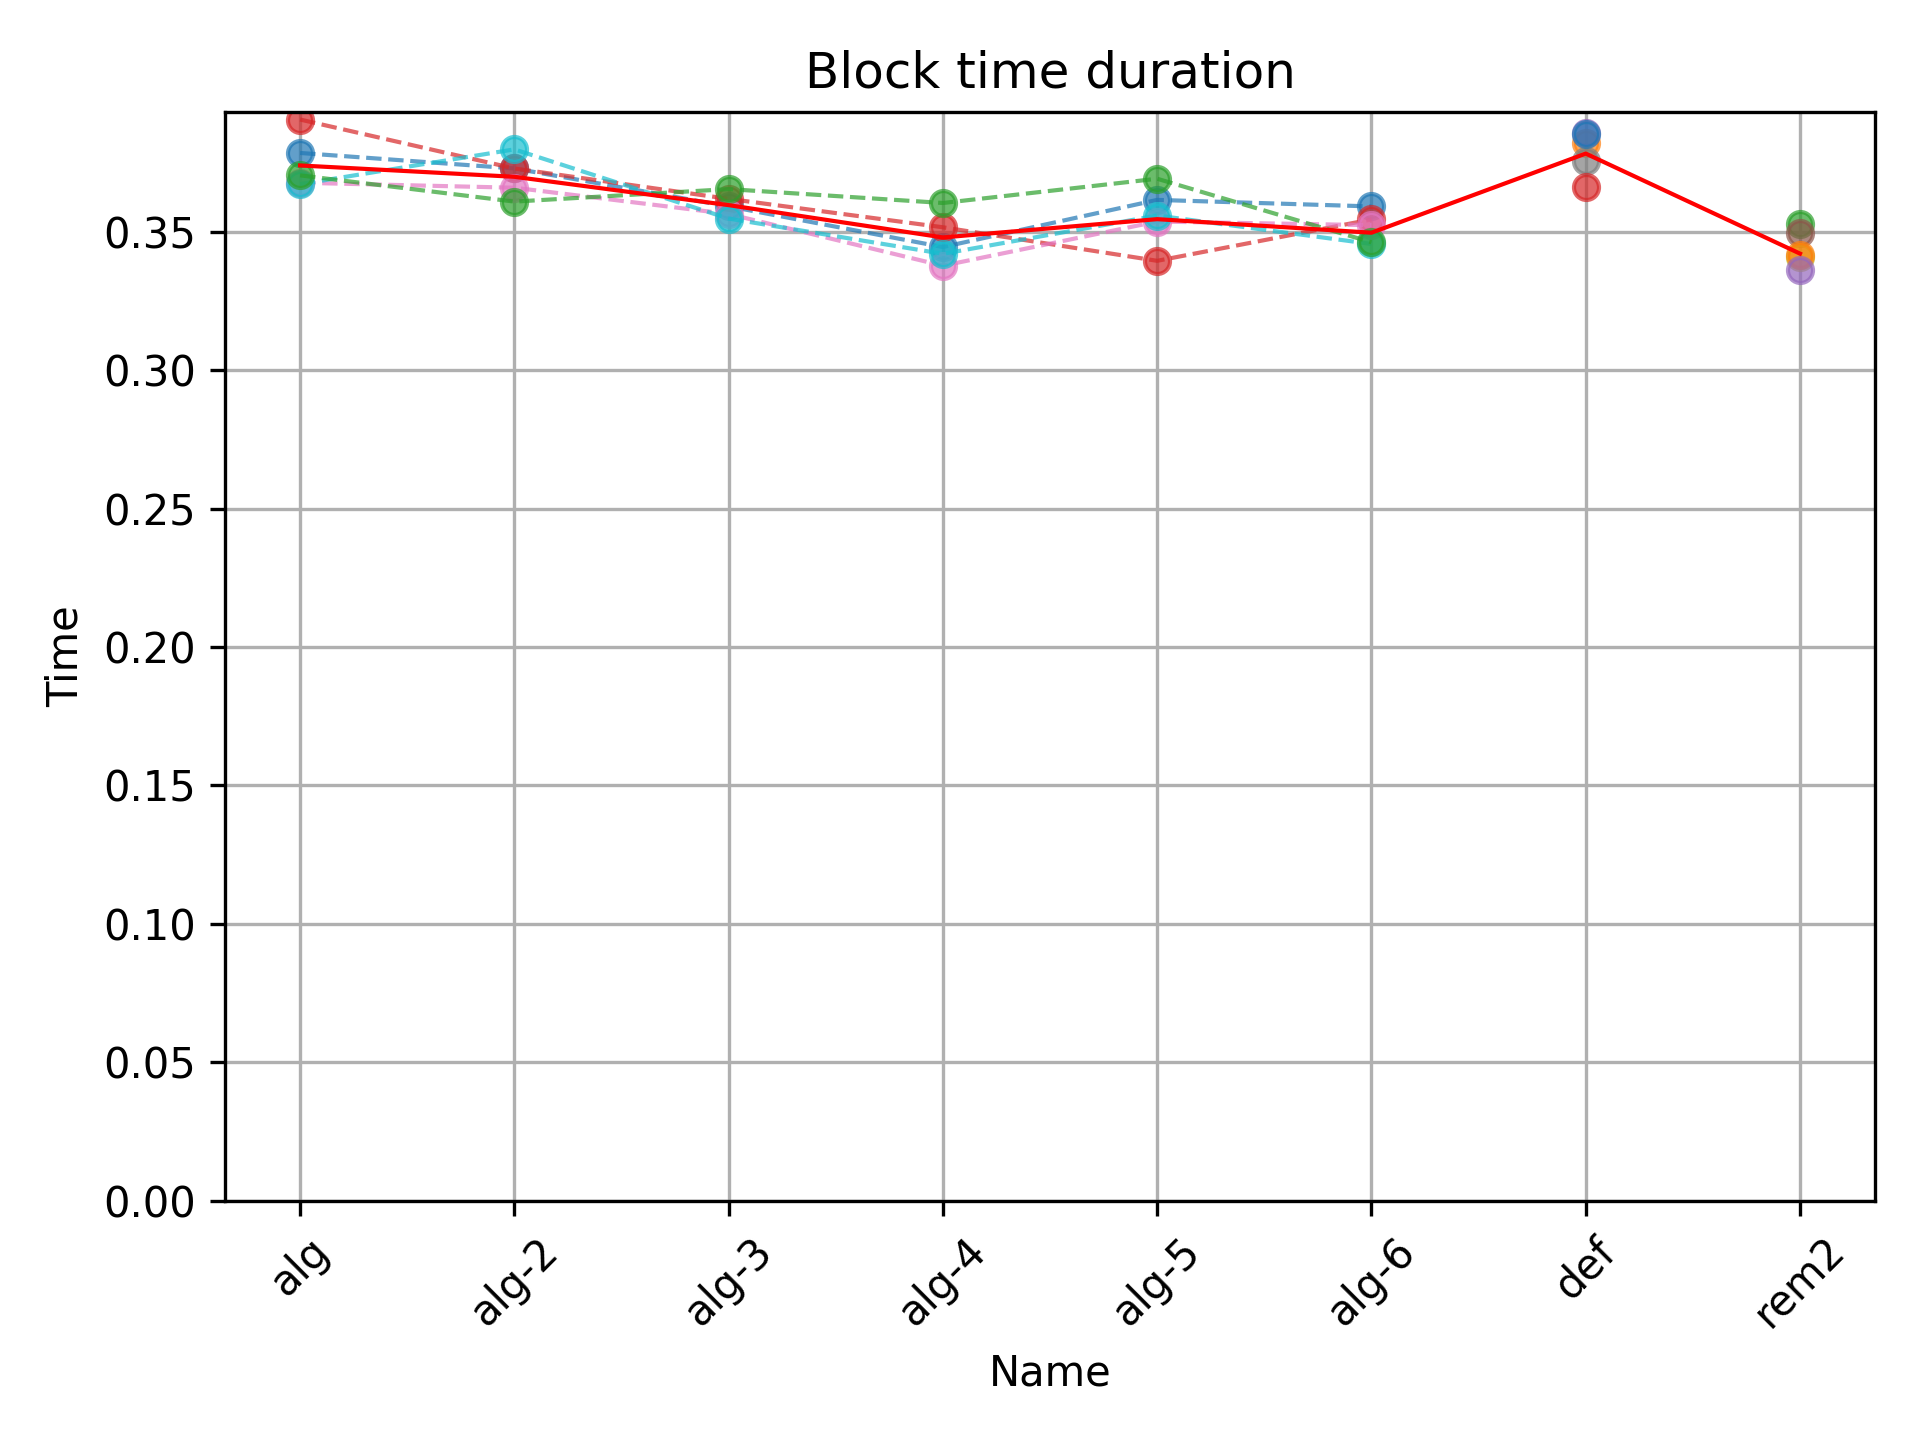
\includegraphics[width=0.3\textwidth]{img/aws13zero.png}}
\caption{Experiment with 24-hour measured 14-node topology from  \cite{di2025impact}.}
\label{alg24}
\end{figure}

\subsubsection{Case C.} Finally, we evaluated a worst-case scenario using a 21-node topology modeled on 16 months of noisy data (\textbf{Fig. \ref{alg3}}). Despite the lack of correlation between latencies of sequential packets, and high latency variability, the algorithm remained robust. It identified subtle patterns to achieve a 6\% gain at the 80th percentile and 3\% at the median without  degrading performance. This stability is crucial for real-world deployment, ensuring that the mechanism provides benefits when patterns exist without introducing overhead during periods of extreme instability.

\begin{figure}[htbp]
\centerline{%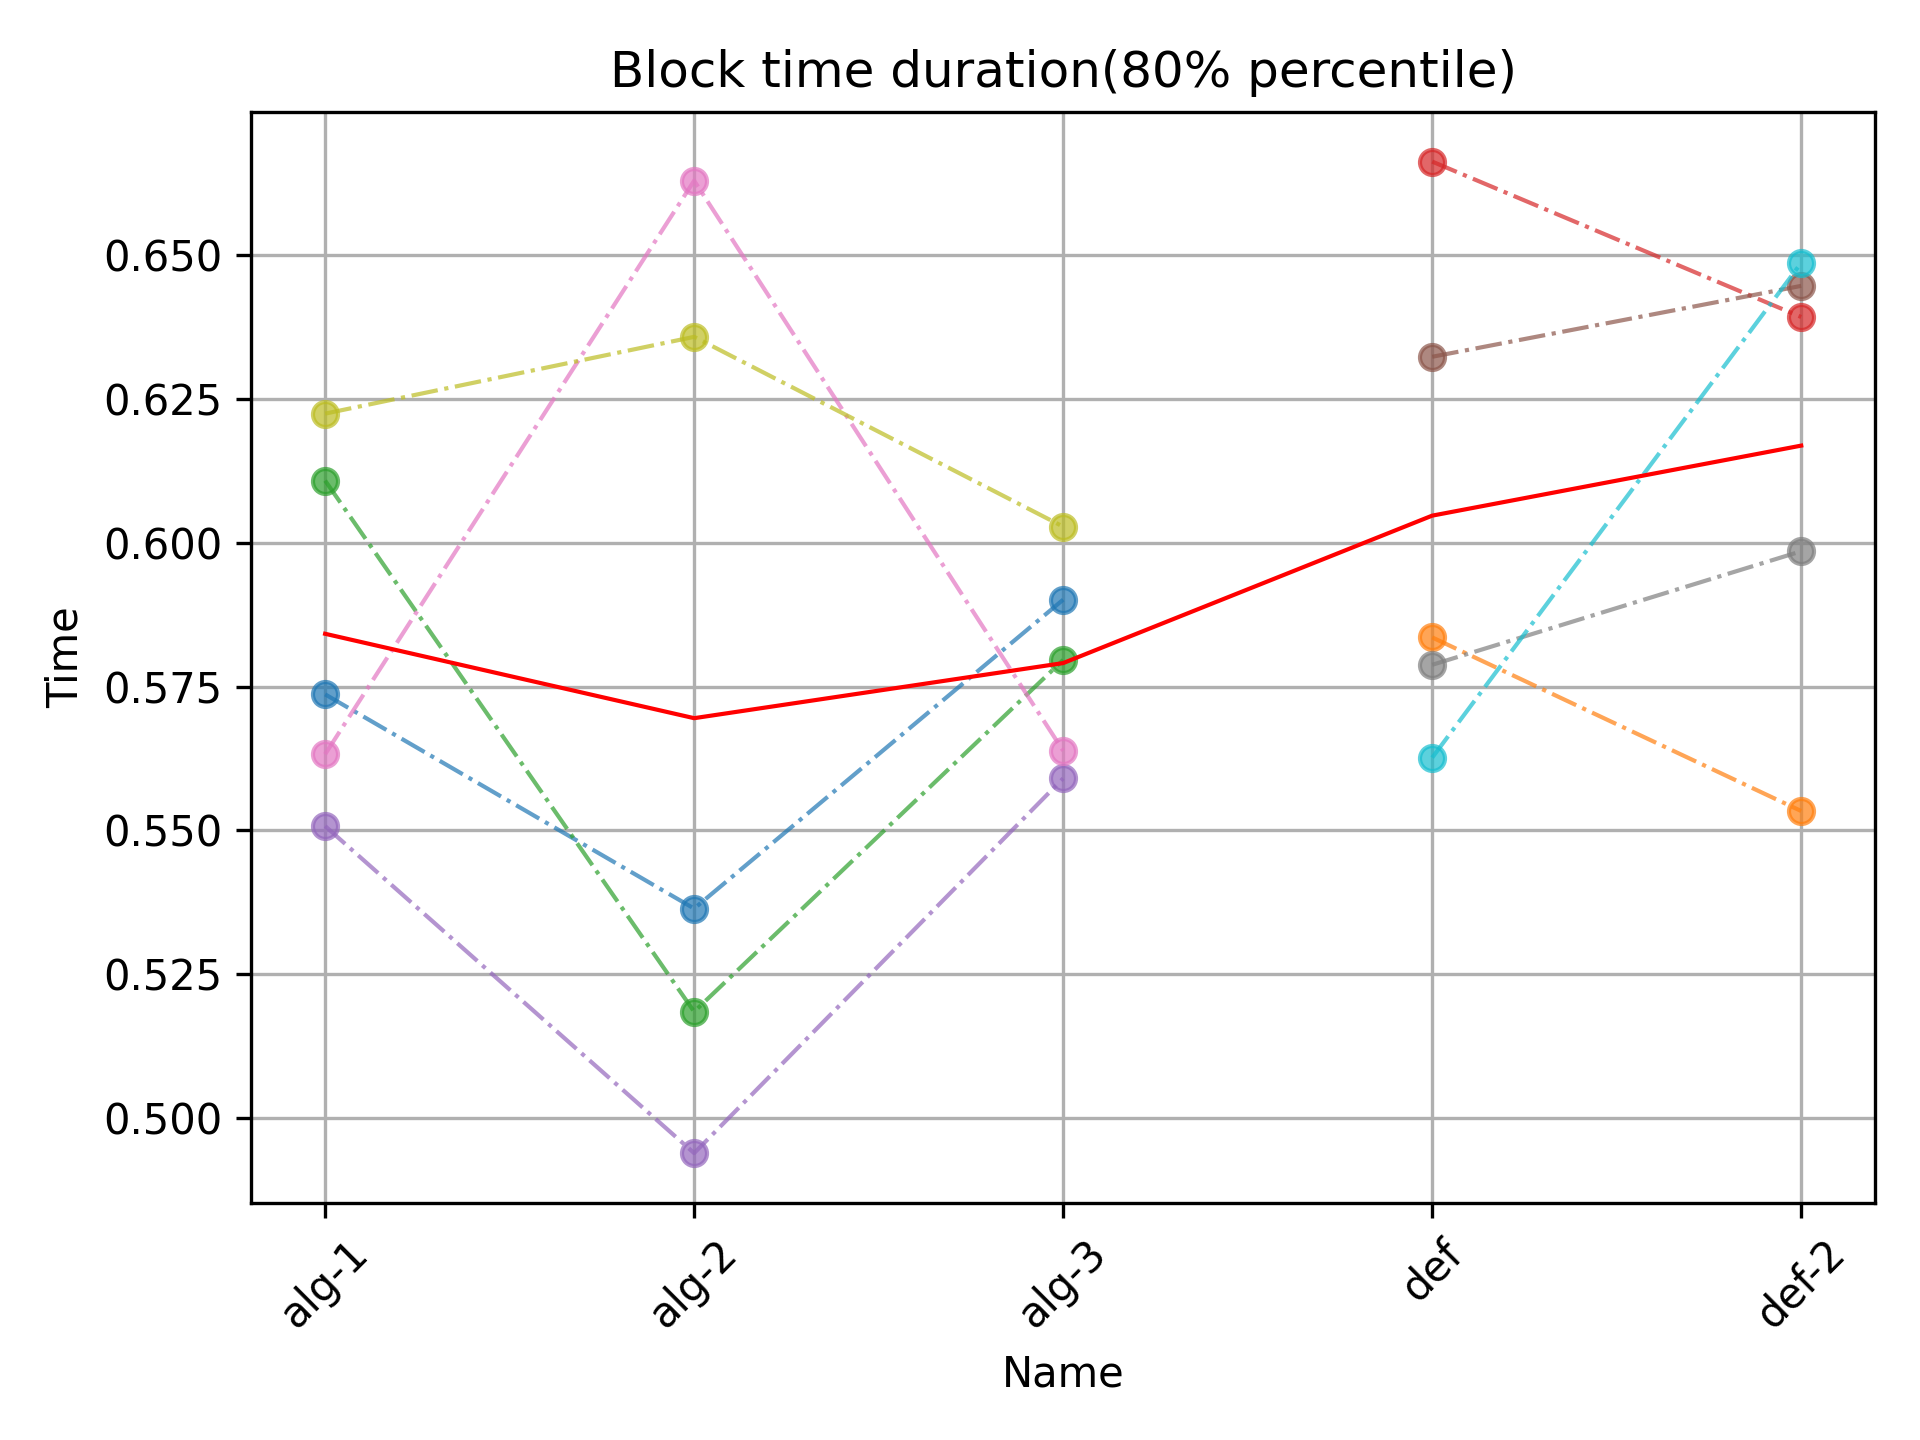
\includegraphics[width=0.3\textwidth]{img/random21.png}}
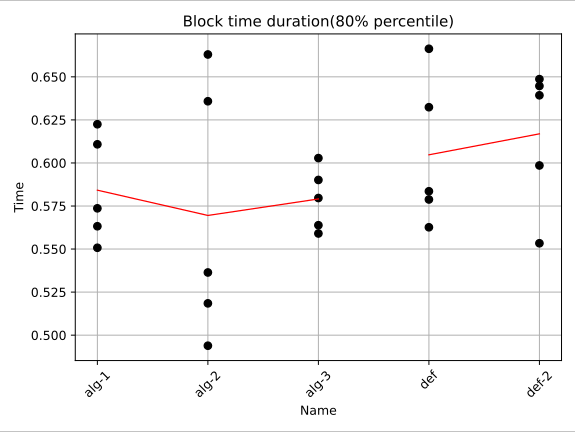
\includegraphics[width=0.6\linewidth]{svgi/rand80th.svg.png}
%\includesvg[width=\linewidth]{svg/rand80th.svg}}
}

%\centerline{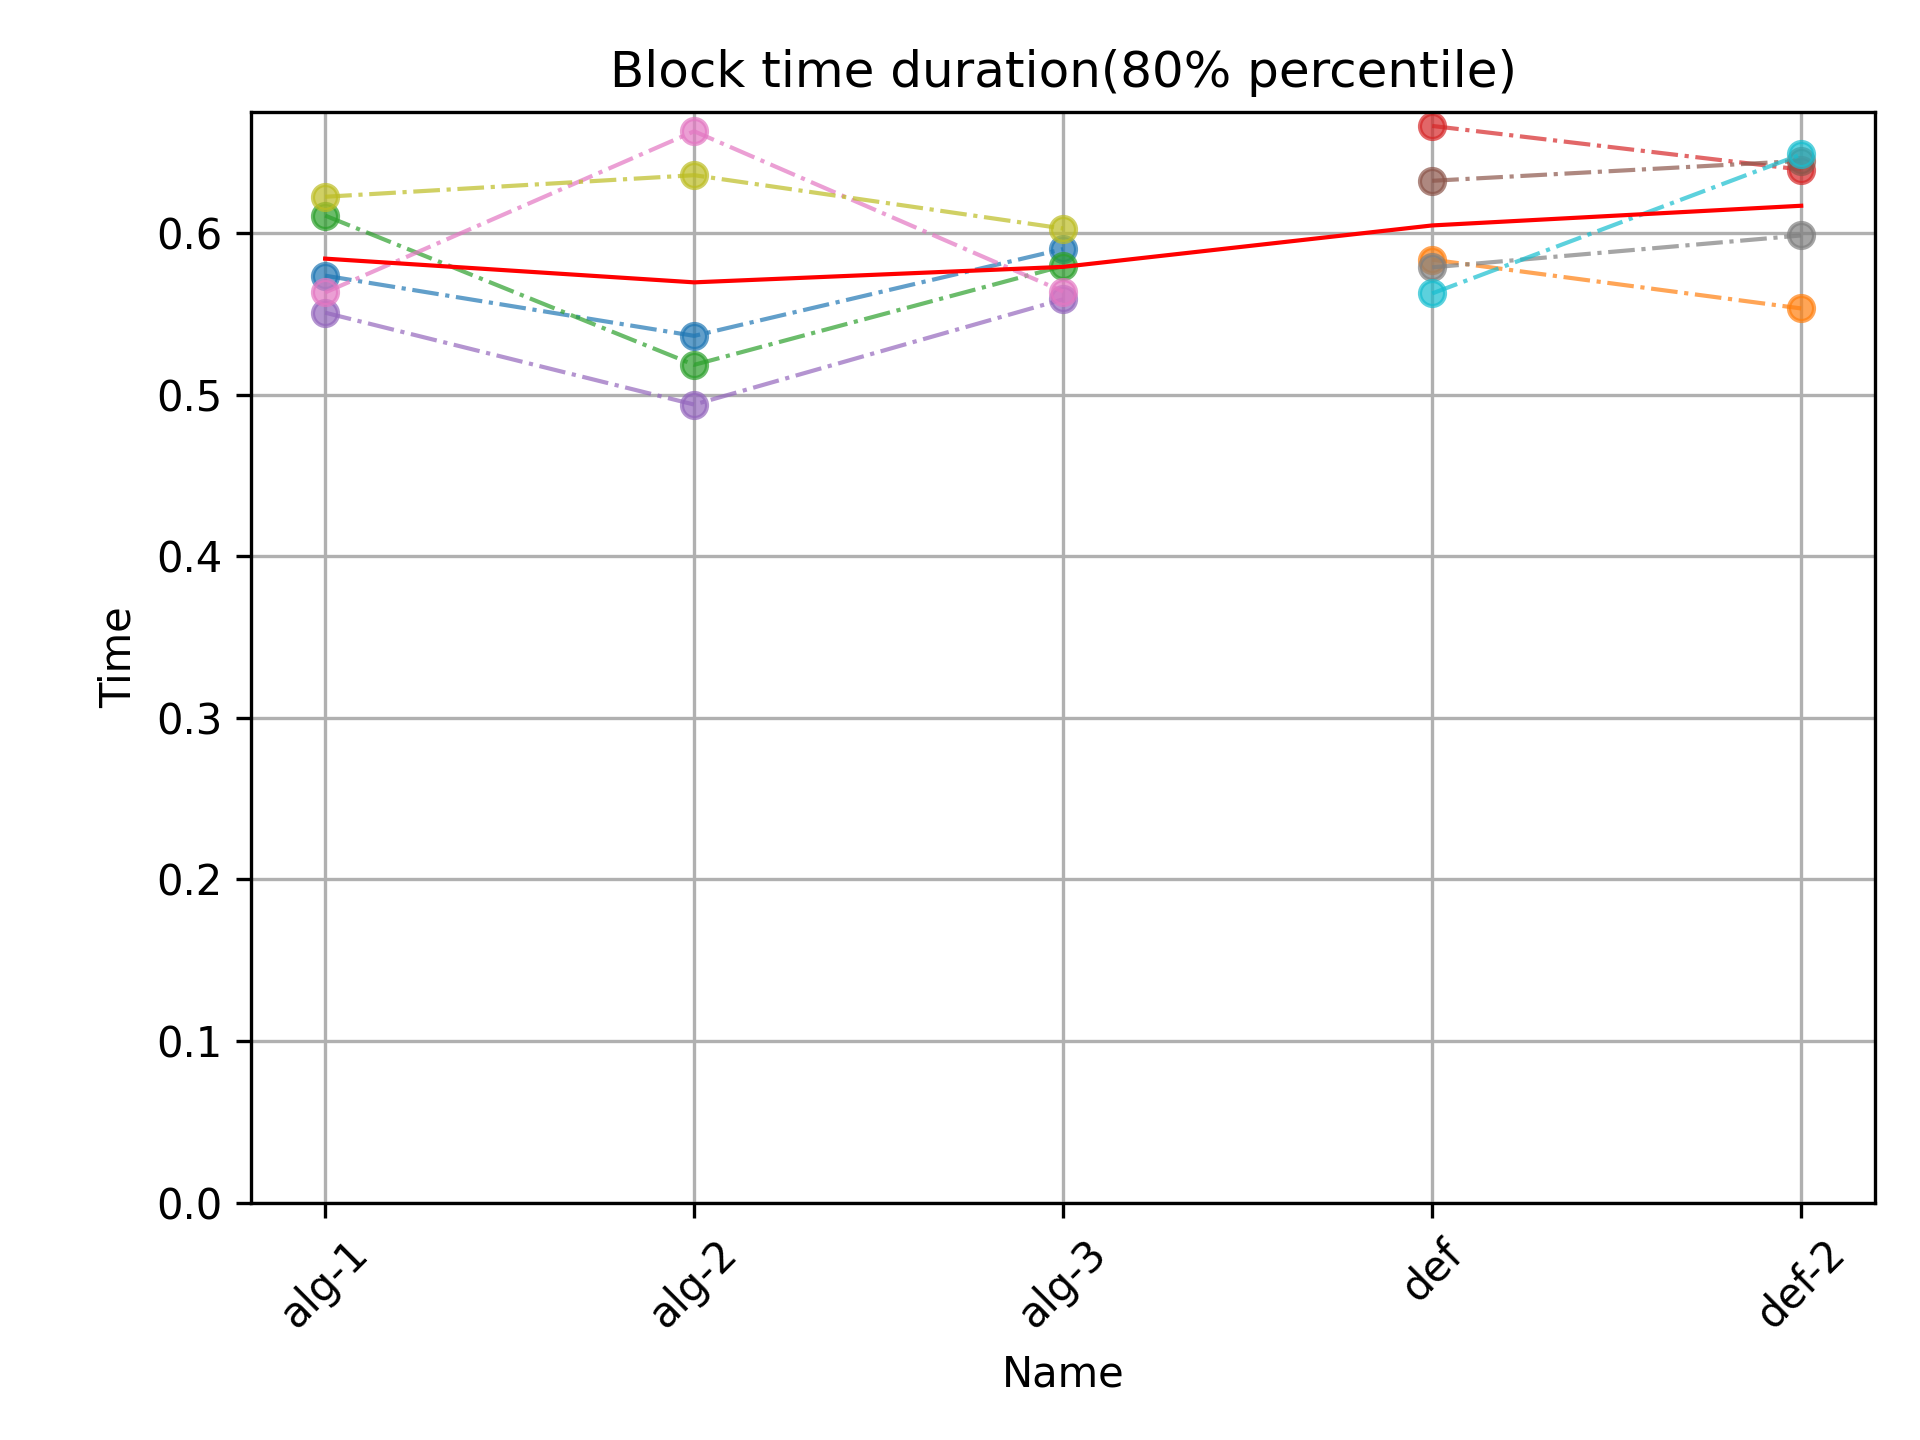
\includegraphics[width=0.3\textwidth]{img/random21zero.png}}
\caption{Experiment with 16 months measures 21 zones topology from \cite{di2025impact}. 5 runs per configuration with 10 rotative runs ????? run run?????}
\label{alg3}
\end{figure}


% \subsection{Multi-instance Evaluation}
% For high-frequency systems where per-instance updates may be excessive, we propose a multi-instance evaluation variant. In this approach, nodes collect local performance observations for $N$ proposals before initiating a distributed consensus on the aggregate results. This modification transforms the score calculation into $S'_n = \beta^N \cdot S_n + \alpha \cdot \sum(L_n)$, where $L_n$ represents a list of $N$ evaluations. This grouping serves two purposes: it significantly reduces the communication overhead and acts as a low-pass filter, smoothing out transient network noise to reveal the underlying performance trends of individual nodes.



% \subsection{Multi-instance Evaluation}

% Noisier topologies or faster systems may not necessitate per-instance update on the score of proposers. In such cases we envision a multi-instance evaluation of proposers, which groups $N$ proposals of a node into a single consensus:

% \begin{enumerate}
%     \item Every time a node $p$ proposes a value, wait for consensus to end and register a local vote.
%     \item Every $N$ times $p$ is the proposer, send the $N$ local votes for the consensus over $p$.
%     \item Reach consensus for each of the $N$ values, defaulting to 0 for impossible consensus (e.g. due to previous nodes leaving the committee).
%     \item After consensus, the network will have a distributed list of values $L_n$ for the node $n$ (e.g. $L_n$ = [-1,-1,0] for $N$=3).
%     \item The network calculates the new value by factoring all $N$ evaluations at once.
% \end{enumerate}

% This turns the previously mentioned $S_n$ calculation into

% $S'_n$ = $\beta^N*Sn + \alpha*sum(L_n)$

% As the vote itself is a simple data structure, for any reasonable choice of $N$ the entire list of votes of a node can fit into a single message. This can further reduce the already small communication cost and also how often consensus happens. A side effect of this is that the larger the $N$ the more is smoothes over any noise in the decisions. This could be useful in networks where nodes exhibit clear performance patterns despite frequent noise.



\section{Discussion and future work}

This paper makes two main contributions. 
First, we experimentally characterize the impact of proposer location on geo-distributed Byzantine consensus. 
Our results show that the proposer is a first-order determinant of consensus performance: its position within the network topology influences not only the duration of the proposal phase itself, but also the composition of quorums and, consequently, the duration of subsequent consensus phases. 
Depending on the topology, the choice of proposer can increase consensus latency by up to 40\%, demonstrating that proposer placement is an important yet often overlooked aspect of geo-distributed deployments.

Second, we introduce a generic performance-aware proposer prioritization mechanism that continuously adapts proposer frequency according to observed consensus performance. 
The mechanism preserves the original Byzantine fault-tolerance guarantees, introduces no additional communication rounds, and can be integrated into existing rotating-leader state machine replication protocols with minimal modifications. 
Although our evaluation focuses on Tendermint, the proposed approach is independent of any specific consensus protocol and is applicable to a broader class of rotating-leader systems.

Several directions remain for future work. 
First, we intend to implement the complete proposer prioritization mechanism within the Malachite codebase and perform a large-scale evaluation. 
Our goal is to deploy experiments on a local cluster with emulated wide-area latencies that reproduce realistic Cosmos network conditions and validator topologies. 
This will allow us to study the behavior of the mechanism at scales approaching production deployments, which may involve committees with up to 180 validators.\footnote{\url{https://docs.cosmos.network/hub/latest/validators/overview}}

Second, a large-scale evaluation will enable us to investigate several open questions that cannot be fully addressed in the current study. 
In particular, we intend to analyze the mechanism's sensitivity to its configuration parameters, evaluate its robustness under dynamic network conditions, and assess the trade-offs between fairness and performance when only a subset of the slowest proposers is deprioritized. 
Such an evaluation will provide a better understanding of the practical limits and benefits of performance-aware proposer selection in real-world blockchain systems.




%In this paper, we study how a proposer's location within a topology affects distributed consensus and propose a generic mechanism to improve performance via leader selection. As our research focuses on Tendermint, further research on other consensus algorithms is warranted to validate these findings and explore potential edge cases. In particular, algorithms such as HotStuff, with its more involved leader, are expected to have more pronounced leader impact on consensus. 
%
%Finally, our mechanism is shown to improve performance with no measurable overhead. Nevertheless, several areas could be explored further, such as the impact of individual parameters and possible improvements. In particular, a more nuanced vote could lead to additional performance improvements. 
%
%
%We intend to modify Malachite to integrate our optimizations and conduct a large-scale performance evaluation, possibly using a local cluster and emulated latencies, to resemble Cosmos.
%
%Cosmos, a large-scale implementation of Tendermint, is expected to have up to 180 nodes in the committee\footnote{\url{https://docs.cosmos.network/hub/latest/validators/overview}}. It is possible that a single fixed proposer could suffer additional overhead at that scale. Nevertheless, reducing the proposer pool to a smaller subset, excluding only the most disproportionally slow nodes, could still be a realistic approach. 




%\begin{credits}
%%\subsubsection{\ackname} A bold run-in heading in small font size at the end of the paper isused for general acknowledgments, for example: This study was funded by X (grant number Y).
%
%\subsubsection{\discintname}
%The authors have no competing interests to declare that are
%relevant to the content of this article. 
%
%\end{credits}


%
% ---- Bibliography ----
%
% BibTeX users should specify bibliography style 'splncs04'.
% References will then be sorted and formatted in the correct style.
%

% \appendix
% \subsection{Proof of Limits of $S'_n$}
% \label{proof}
% The value $S'_n$, respective to the updated score of the node $n$, is modified follows: 

% $S'_n = \beta*S_n+\alpha*decided_n$

% where $S_n$ is the previous score, $0\le\beta<1$, $\alpha\ge0$, and $decided_n \in \{-1,0,1\}$.

% The value reaches its maximum when, for every decision, $decided_n=1$, and minimum when $decided_n=-1$. 

% For clarity, we omit the multiplication symbol and denote $S_n$ by $S$, with $S_0$ representing the initial state (always 0), and $S_1$ being the next iteration until an infinite $S_N$. This leads to the following recursion representing the limits of the value $S'_n$:

% $S_N = \beta S_{N-1}+\alpha$

% Where $\alpha$ is implicitly multiplied by a constant $decided_n \in \{1,-1\}$. We then expand the function to determine its limit as follows:
% \begin{enumerate}
%     \item Expansion of the recursion\\
% $S_N = \beta S_{N-1}+\alpha$ \\
% $S_N = \beta(\beta S_{N-2}+\alpha)+\alpha$\\
% $S_N = \beta^2S_{N-2}+\beta\alpha+\alpha$\\
% $S_N = \beta^2(\beta S_{N-3} +\alpha)+\beta\alpha+\alpha$\\
% $S_N = \beta^3S_{N-3}+\beta^2\alpha+\beta\alpha+\alpha$\\
% Iterating this process yields\\$S_N=\beta S_0+\alpha(1+\beta+\beta^2+...+\beta^{N-1})$\\ 
% Since $S_0$, the initial state, is zero, we can reduce $S_N$ into $\alpha(1+\beta+\beta^2+...+\beta^{N-1})$ 
% \item Closed form solution \\
% We define $s$ as the geometric series $(1+\beta+...+\beta^{N-1})$. We then derive its closed-form expression as follows:\\
% $s=1+\beta¹+...+\beta^{N-1}$\\
% $\beta s=\beta¹+\beta^2+...+\beta^{N}$\\
% $s-\beta s=(1+\beta+...+\beta^{N-1})-(\beta+...+\beta^{N-1}+\beta^N)$\\
% $s-\beta s=1-\beta^N$\\
% $s(1-\beta)=1-\beta^N$\\
% $s=\frac{1-\beta^N}{1-\beta}$
% \item Taking the limit\\
% We can now substitute the geometric series for the closed-form expression, yielding\\
% $S_N=\alpha(\frac{1-\beta^N}{1-\beta})$\\
% For $0 \le\beta <1$, we have $\lim\limits_{N\to\infty} \beta^N=0$, therefore, \[\lim_{N\to\infty}S_N=\frac{\alpha}{1-\beta}\]

% Multiplying $\alpha$ by a $decided_n\in\{1,-1\}$ yields the corresponding upper and lower limits. 
% \end{enumerate}

\bibliographystyle{splncs04}
\bibliography{references}

\end{document}

\begin{thebibliography}{8}
\bibitem{ref_article1}
Author, F.: Article title. Journal \textbf{2}(5), 99--110 (2016)

\bibitem{ref_lncs1}
Author, F., Author, S.: Title of a proceedings paper. In: Editor,
F., Editor, S. (eds.) CONFERENCE 2016, LNCS, vol. 9999, pp. 1--13.
Springer, Heidelberg (2016). \doi{10.10007/1234567890}

\bibitem{ref_book1}
Author, F., Author, S., Author, T.: Book title. 2nd edn. Publisher,
Location (1999)

\bibitem{ref_proc1}
Author, A.-B.: Contribution title. In: 9th International Proceedings
on Proceedings, pp. 1--2. Publisher, Location (2010)

\bibitem{ref_url1}
LNCS Homepage, \url{http://www.springer.com/lncs}, last accessed 2023/10/25
\end{thebibliography}
\end{document}



\section{First Section}
\subsection{A Subsection Sample}
Please note that the first paragraph of a section or subsection is
not indented. The first paragraph that follows a table, figure,
equation etc. does not need an indent, either.

Subsequent paragraphs, however, are indented.

\subsubsection{Sample Heading (Third Level)} Only two levels of
headings should be numbered. Lower level headings remain unnumbered;
they are formatted as run-in headings.

\paragraph{Sample Heading (Fourth Level)}
The contribution should contain no more than four levels of
headings. Table~\ref{tab1} gives a summary of all heading levels.

\begin{table}
\caption{Table captions should be placed above the
tables.}\label{tab1}
\begin{tabular}{|l|l|l|}
\hline
Heading level &  Example & Font size and style\\
\hline
Title (centered) &  {\Large\bfseries Lecture Notes} & 14 point, bold\\
1st-level heading &  {\large\bfseries 1 Introduction} & 12 point, bold\\
2nd-level heading & {\bfseries 2.1 Printing Area} & 10 point, bold\\
3rd-level heading & {\bfseries Run-in Heading in Bold.} Text follows & 10 point, bold\\
4th-level heading & {\itshape Lowest Level Heading.} Text follows & 10 point, italic\\
\hline
\end{tabular}
\end{table}


\noindent Displayed equations are centered and set on a separate
line.
\begin{equation}
x + y = z
\end{equation}
Please try to avoid rasterized images for line-art diagrams and
schemas. Whenever possible, use vector graphics instead (see
Fig.~\ref{fig1}).

\begin{figure}
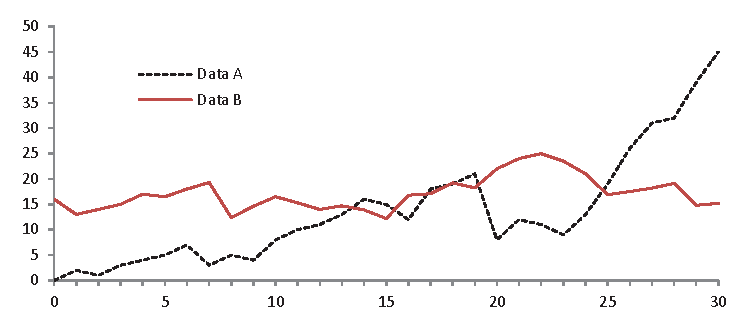
\includegraphics[width=\textwidth]{fig1.eps}
\caption{A figure caption is always placed below the illustration.
Please note that short captions are centered, while long ones are
justified by the macro package automatically.} \label{fig1}
\end{figure}

\begin{theorem}
This is a sample theorem. The run-in heading is set in bold, while
the following text appears in italics. Definitions, lemmas,
propositions, and corollaries are styled the same way.
\end{theorem}
%
% the environments 'definition', 'lemma', 'proposition', 'corollary',
% 'remark', and 'example' are defined in the LLNCS documentclass as well.
%

For citations of references, we prefer the use of square brackets
and consecutive numbers. Citations using labels or the author/year
convention are also acceptable. The following bibliography provides
a sample reference list with entries for journal
articles~\cite{ref_article1}, an LNCS chapter~\cite{ref_lncs1}, a
book~\cite{ref_book1}, proceedings without editors~\cite{ref_proc1},
and a homepage~\cite{ref_url1}. Multiple citations are grouped
\cite{ref_article1,ref_lncs1,ref_book1},
\cite{ref_article1,ref_book1,ref_proc1,ref_url1}.